\chapter{Resultados}
\label{cap:resultados}

A continuación se presentan los resultados obtenidos con los métodos creados junto a sus métricas asociadas, así como también se presentan las comparaciones relacionadas a otros métodos tanto para los conjuntos de datos simulados como los reales. 

\section{Datos simulados}

\subsection{Self-calibration}

\subsubsection{\textit{Long-baseline}}

La prueba de \textit{self-calibration} utiliza el conjunto de datos simulado creado en la sección \ref{sec:simulated_data}, sin embargo estas vienen perturbadas por una ganancia aleatoria que está asignada a una antena, donde la imagen resultante de esta puede ser vista en la Figura \ref{fig:noisy_image}. Cabe destacar que los datos perturbados son aquellos asociados a una antena de referencia, que para el caso del conjunto de datos reducidos de HD163296 sería la antena DA48, así como también se considera todos los parámetros proporcionados por los scripts que se pueden encontrar en el sitio web de DSHARP, específicamente el asociado al conjunto de datos HD163296. 

\begin{figure}[!ht]
 \centering
  \subfloat[Original]{
   \label{fig:noisy_original}
    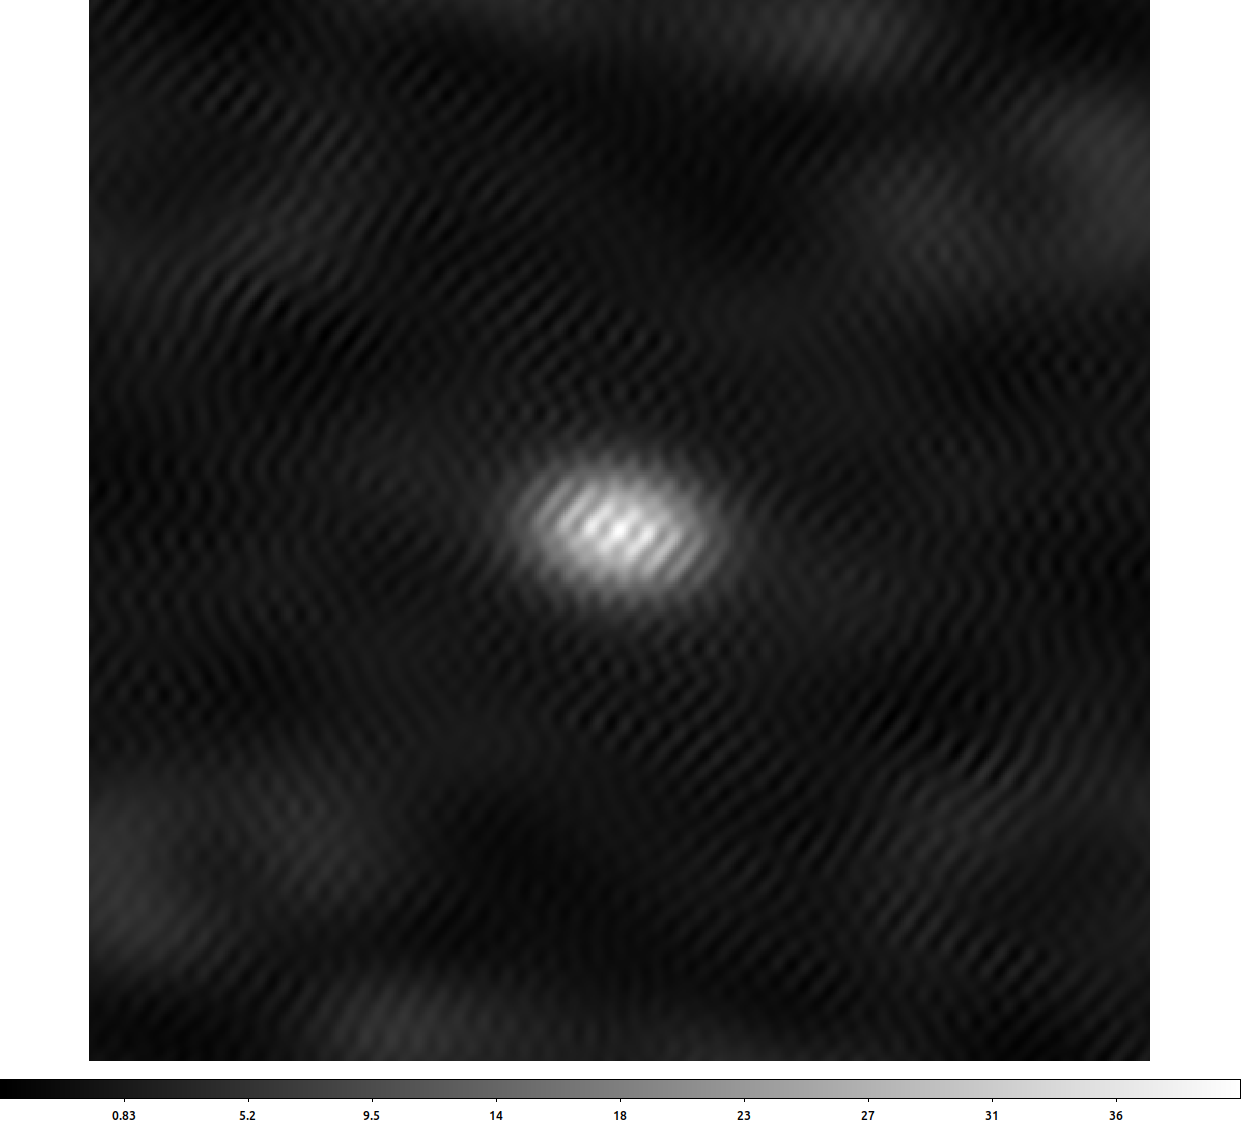
\includegraphics[width=0.45\textwidth]{images/noisy_dataset_dirty.png}}
  \subfloat[Color]{
   \label{fig:noisy_color}
    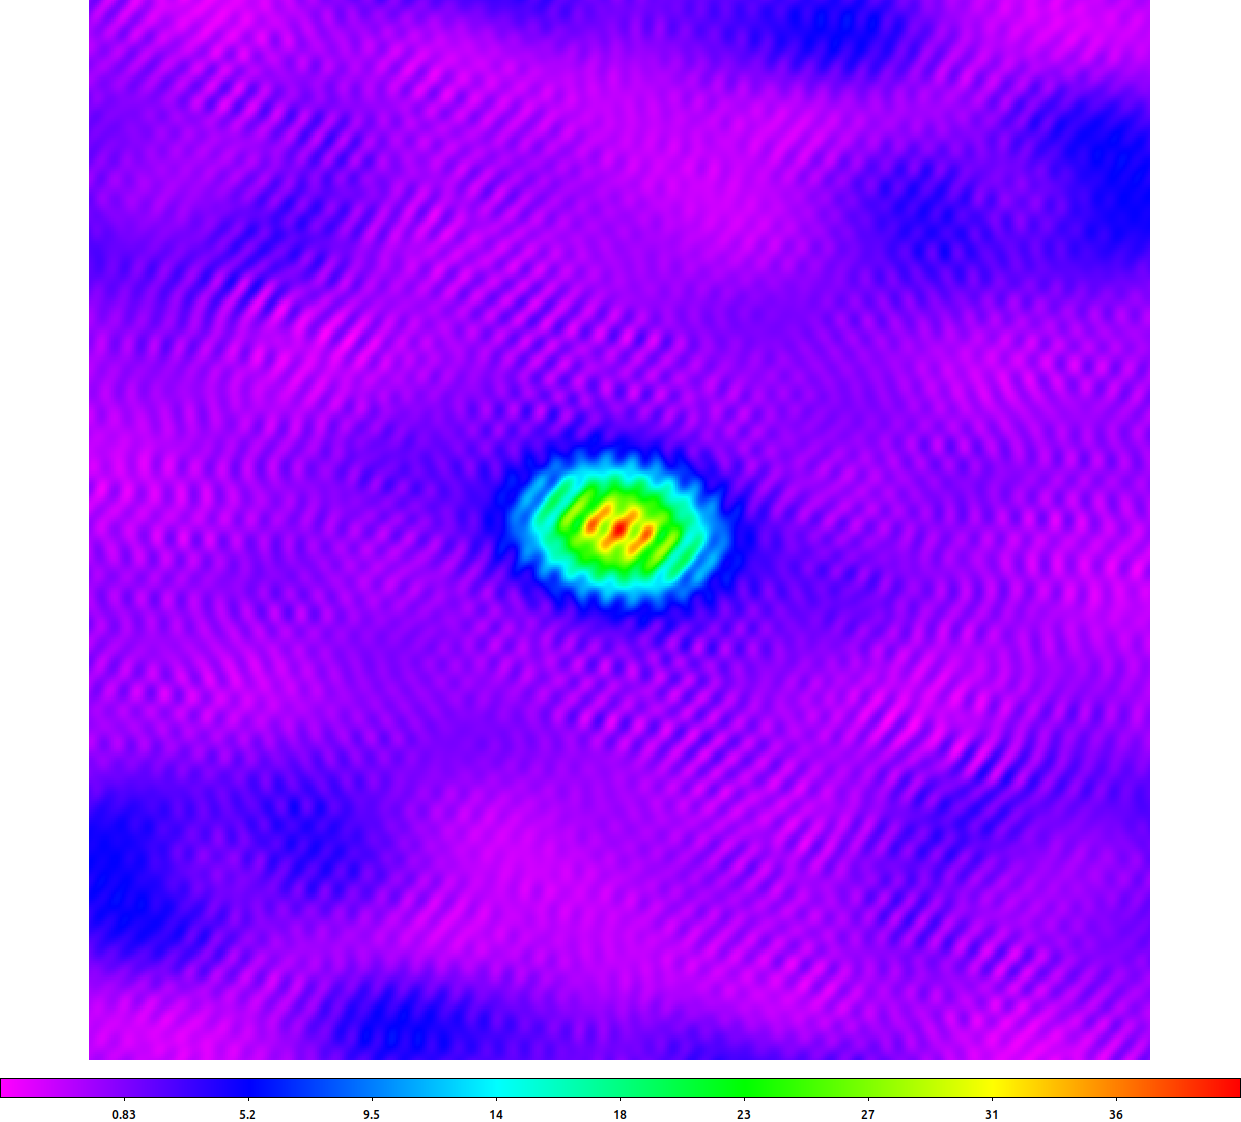
\includegraphics[width=0.45\textwidth]{images/noisy_dataset_dirty_color.png}}
 \caption[Imagen simulado afectada por una fase (\textit{long-baseline})]{Imagen simulado afectada por una fase (\textit{long-baseline}). Fuente: Elaboración propia.}
 \label{fig:noisy_image}
\end{figure}

La síntesis de imágenes es realizada a través de los algoritmos de CLEAN y MEM a través de las herramientas CASA y GPUVMEM. En este momento no se considera la ejecución del algoritmo \textit{Bispectrum} debido a que en esta sección se desea mostrar la eficacia del algoritmo para \textit{self-calibration} desarrollado. 

Para la primera iteración se realiza una calibración de fase considerando un rango de tiempo de 360 segundos. En la figura \ref{fig:phasecal_1iter} se observa el resultado obtenido luego de realizar el método CLEAN al conjunto de datos calibrado donde este obtuvo un valor de PSNR de 218.1818 y un NRMSE de 0.986209. Por otro lado, en la Figura \ref{fig:phasecal_1iter_gpuvmem} se observa el resultado luego de realizar el método MEM sobre el conjunto de datos calibrado, obteniendo así un PSNR de 219.3238 y un NRMSE 0.705504.

\begin{figure}[!ht]
 \centering
  \subfloat[Original]{
   \label{fig:clean_original_clean_1iter}
    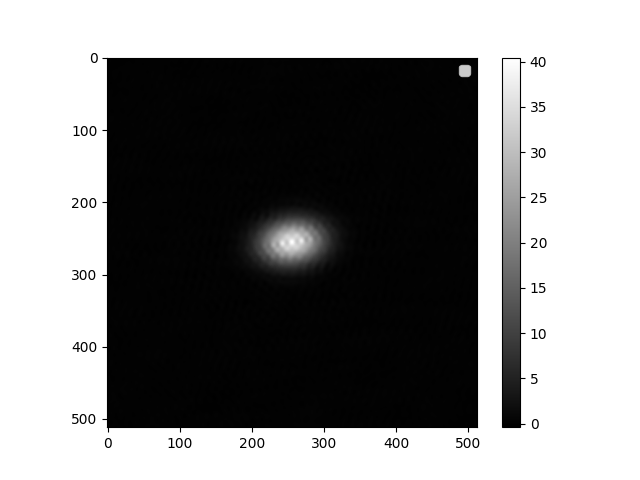
\includegraphics[width=0.5\textwidth]{images/sim_p0_long.png}}
  \subfloat[Color]{
   \label{fig:clean_original_color_1iter}
    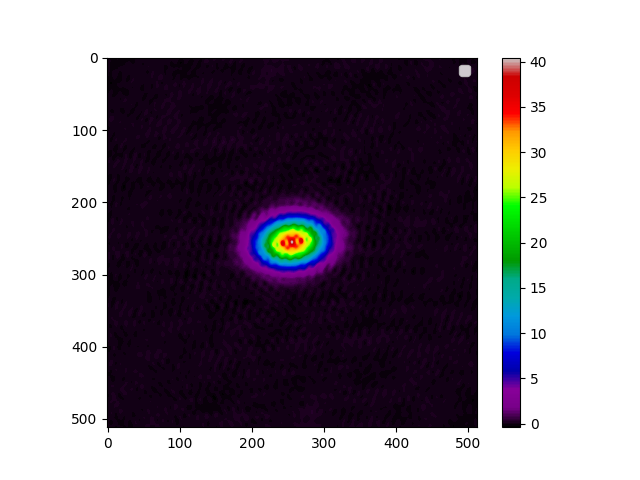
\includegraphics[width=0.5\textwidth]{images/sim_p0_long_color.png}}
    \vspace{0.3cm}
  \subfloat[Residuos Original]{
   \label{fig:clean_residual_clean_1iter}
    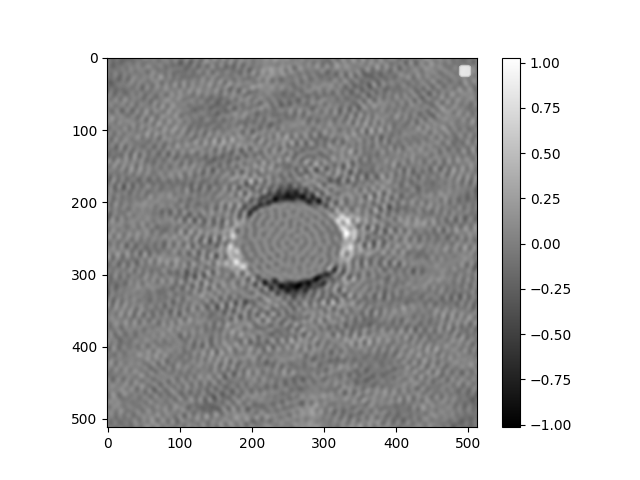
\includegraphics[width=0.5\textwidth]{images/sim_p0_long_residual.png}}
  \subfloat[Residuos Color]{
   \label{fig:clean_resisdual_color_1iter}
    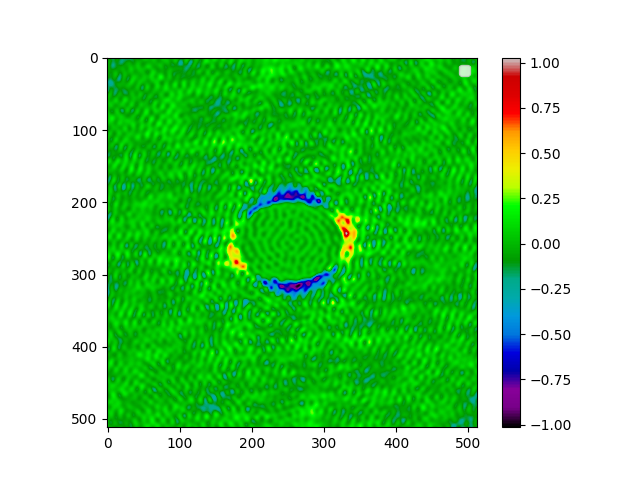
\includegraphics[width=0.5\textwidth]{images/sim_p0_long_color_residual.png}}
 \caption[Primera iteración para conjunto de datos simulado CLEAN (\textit{long-baseline})]{Primera iteración para conjunto de datos simulado CLEAN (\textit{long-baseline}). Fuente: Elaboración propia.}
 \label{fig:phasecal_1iter}
\end{figure}

\begin{figure}[!ht]
 \centering
  \subfloat[Original]{
   \label{fig:gpuvmem_original_1iter}
    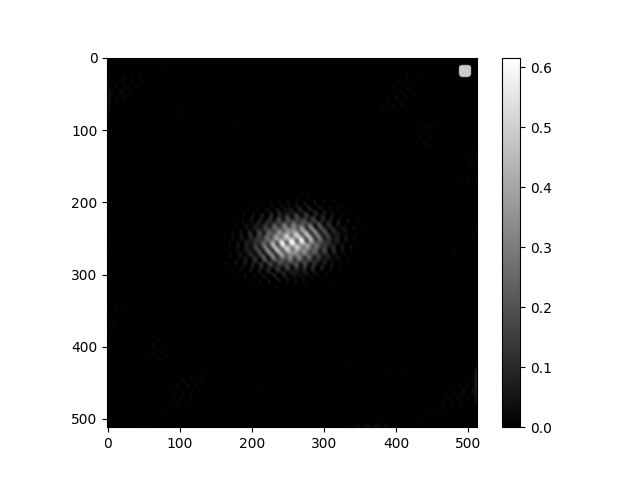
\includegraphics[width=0.5\textwidth]{images/sim_p0_long_gpuvmem.png}}
  \subfloat[Color]{
   \label{fig:gpuvmem_color_1iter}
    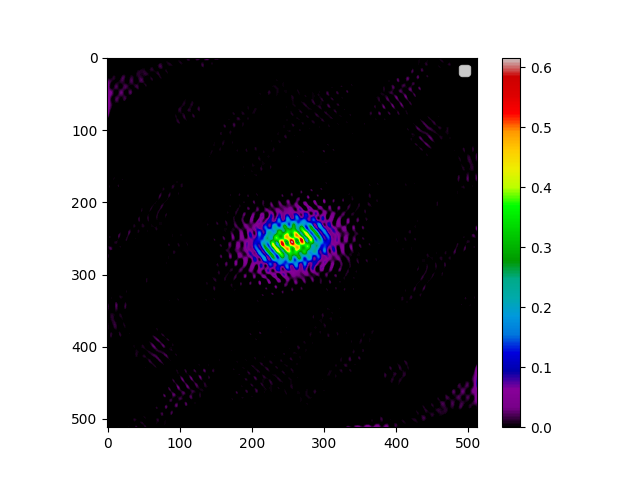
\includegraphics[width=0.5\textwidth]{images/sim_p0_long_gpuvmem_color.png}}
    \vspace{0.3cm}
  \subfloat[Original]{ 
   \label{fig:gpuvmem_residual_original_1iter}
    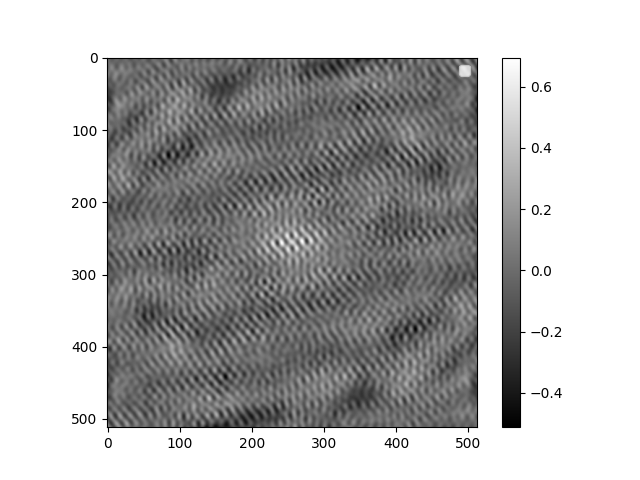
\includegraphics[width=0.5\textwidth]{images/sim_p0_long_gpuvmem_residual.png}}
  \subfloat[Color]{
   \label{fig:gpuvmem_residual_color_1iter}
    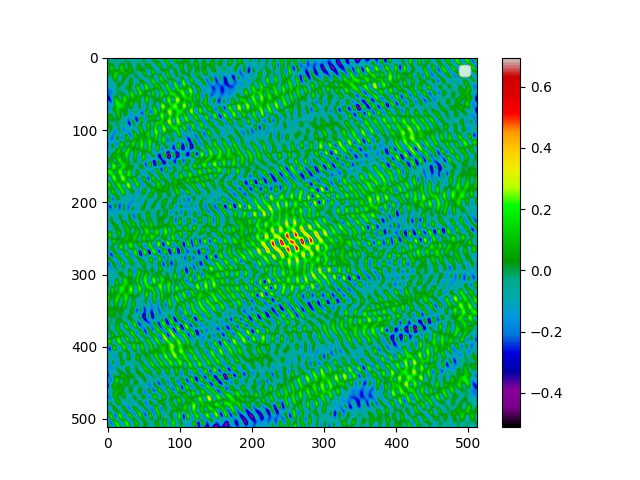
\includegraphics[width=0.5\textwidth]{images/sim_p0_long_gpuvmem_color_residual.png}}
 \caption[Primera iteración para conjunto de datos simulado GPUVMEM (\textit{long-baseline})]{Primera iteración para conjunto de datos simulado GPUVMEM (\textit{long-baseline}). Fuente: Elaboración propia.}
 \label{fig:phasecal_1iter_gpuvmem}
\end{figure}

Una segunda iteración de fase se realiza con un rango de tiempo de 120 segundos considerando la misma antena de referencia. En la Figura \ref{fig:phasecal_2iter} se puede ver el resultado obtenido con el método CLEAN al aplicarse en el conjunto nuevamente calibrado, donde este obtuvo un PSNR de 224.1047 y un NRMSE de 0.986204, en cambio, la Figura \ref{fig:phasecal_2iter_gpuvmem} muestra el resultado con el método MEM donde este obtuvo un PSNR de 218.4566 y un NRMSE de 0.706291. 

\begin{figure}[!ht]
 \centering
  \subfloat[Original]{
   \label{fig:clean_original_clean_2iter}
    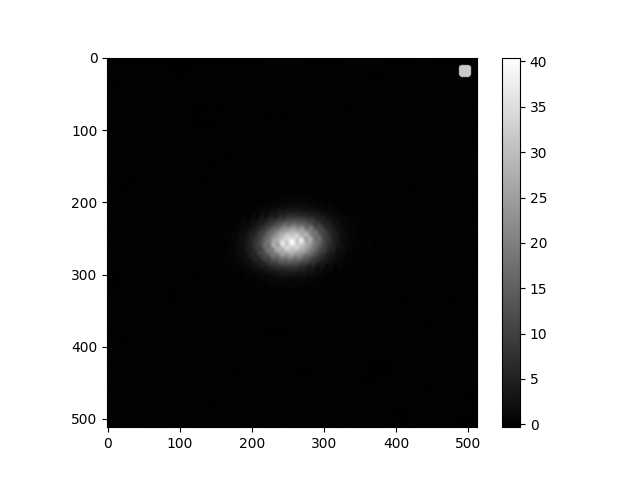
\includegraphics[width=0.5\textwidth]{images/sim_p1_long.png}}
  \subfloat[Color]{
   \label{fig:clean_original_color_2iter}
    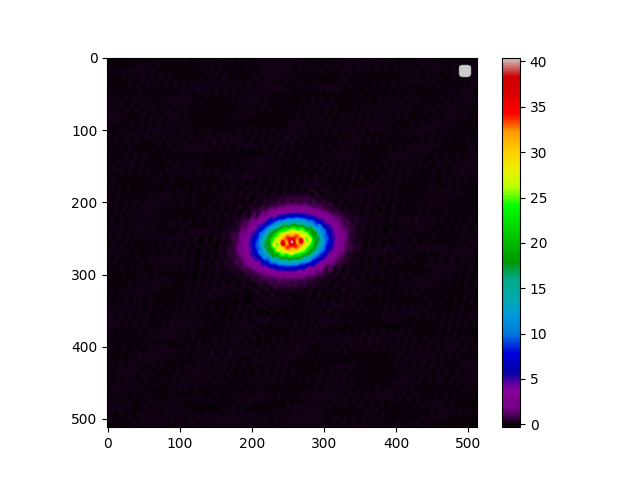
\includegraphics[width=0.5\textwidth]{images/sim_p1_long_color.png}}
    \vspace{0.3cm}
  \subfloat[Residuos Original]{
   \label{fig:clean_residual_clean_2iter}
    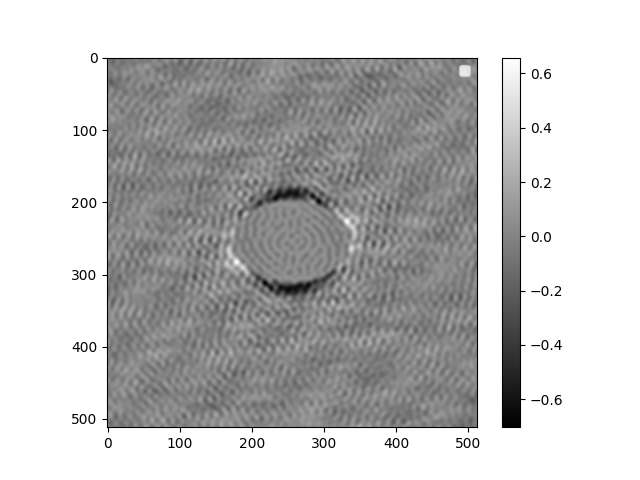
\includegraphics[width=0.5\textwidth]{images/sim_p1_long_residual.png}}
  \subfloat[Residuos Color]{
   \label{fig:clean_residual_color_2iter}
    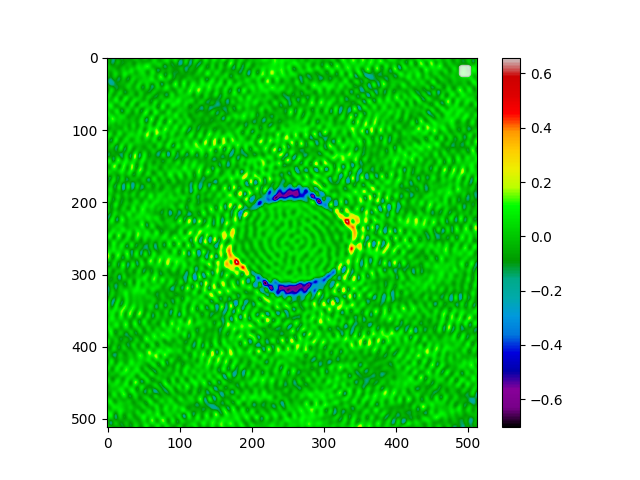
\includegraphics[width=0.5\textwidth]{images/sim_p1_long_color_residual.png}}
 \caption[Segunda iteración para conjunto de datos simulado CLEAN (\textit{long-baseline})]{Segunda iteración para conjunto de datos simulado CLEAN (\textit{long-baseline}). Fuente: Elaboración propia.}
 \label{fig:phasecal_2iter}
\end{figure}

\begin{figure}[!ht]
 \centering
  \subfloat[Original]{
   \label{fig:gpuvmem_original_2iter}
    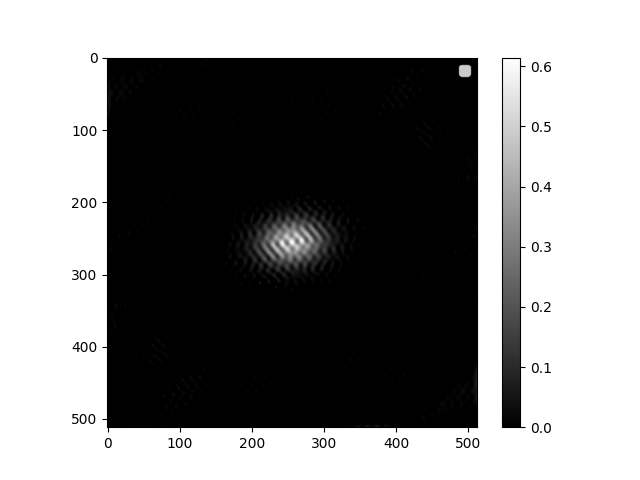
\includegraphics[width=0.5\textwidth]{images/sim_p1_long_gpuvmem.png}}
  \subfloat[Color]{
   \label{fig:gpuvmem_color_2iter}
    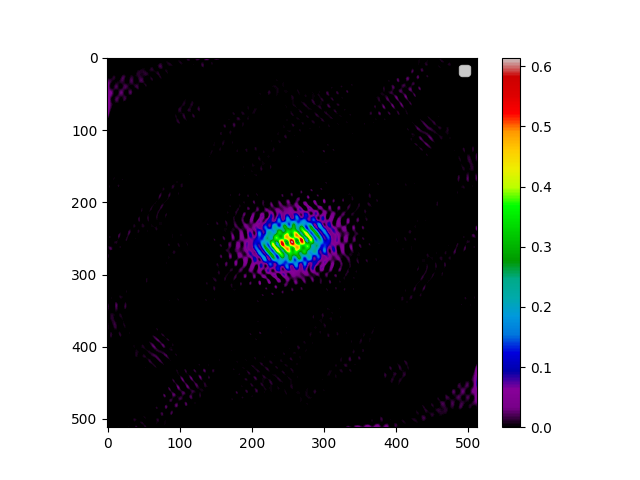
\includegraphics[width=0.5\textwidth]{images/sim_p1_long_gpuvmem_color.png}}
    \vspace{0.3cm}
    \subfloat[Residuo Original]{
   \label{fig:gpuvmem_original_2iter_residual}
    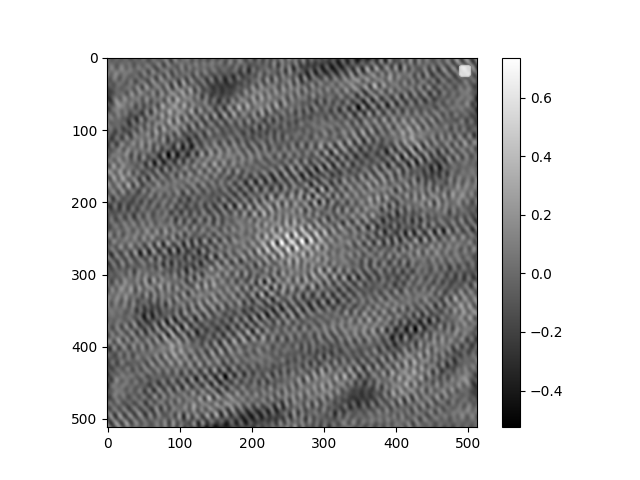
\includegraphics[width=0.5\textwidth]{images/sim_p1_long_gpuvmem_residual.png}}
  \subfloat[Residuo Color]{
   \label{fig:gpuvmem_color_2iter_residual}
    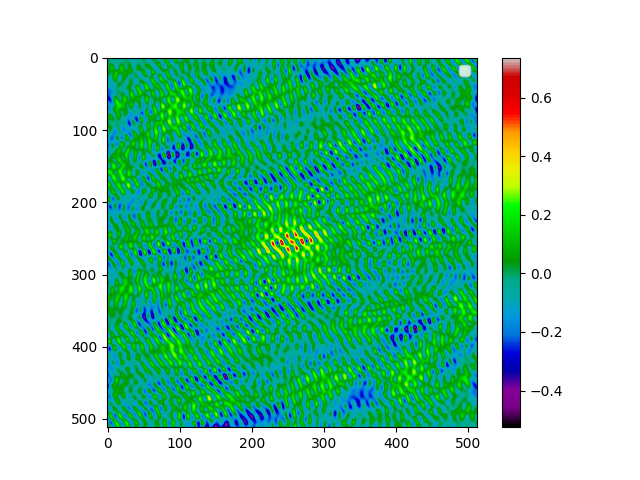
\includegraphics[width=0.5\textwidth]{images/sim_p1_long_gpuvmem_color_residual.png}}
 \caption[Segunda iteración para conjunto de datos simulado GPUVMEM (\textit{long-baseline})]{Segunda iteración para conjunto de datos simulado GPUVMEM (\textit{long-baseline}). Fuente: Elaboración propia.}
 \label{fig:phasecal_2iter_gpuvmem}
\end{figure}

La tercera iteración se realiza el \textit{self-calibration} de fase, considerando un tiempo de 60 segundos con la misma antena de referencia que las antenas anteriores. La Figura \ref{fig:phasecal_3iter} y la Figura \ref{fig:phasecal_3iter_gpuvmem} muestran los valores obtenidos con los métodos de CLEAN y MEM respectivamente, donde la primera obtuvo un PSNR de 217.3753 y un NRMSE de 0.985206, en cambio la otra obtuvo un PSNR de 218.0049  y un NRMSE de 0.706730.  

\begin{figure}[!ht]
 \centering
  \subfloat[Original]{
   \label{fig:clean_original_clean_3iter}
    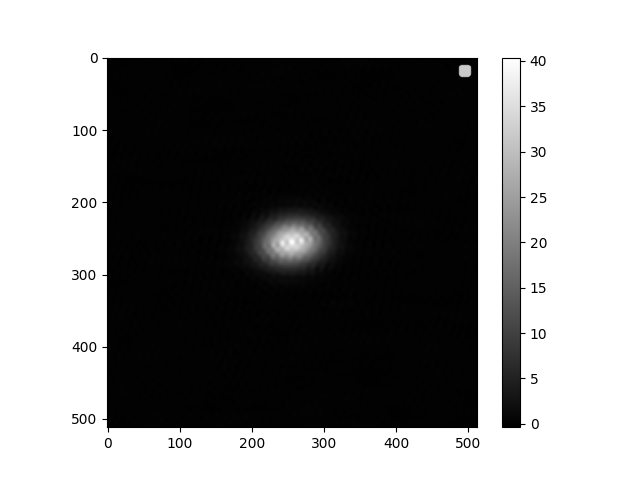
\includegraphics[width=0.5\textwidth]{images/sim_p2_long.png}}
  \subfloat[Color]{
   \label{fig:clean_original_color_3iter}
    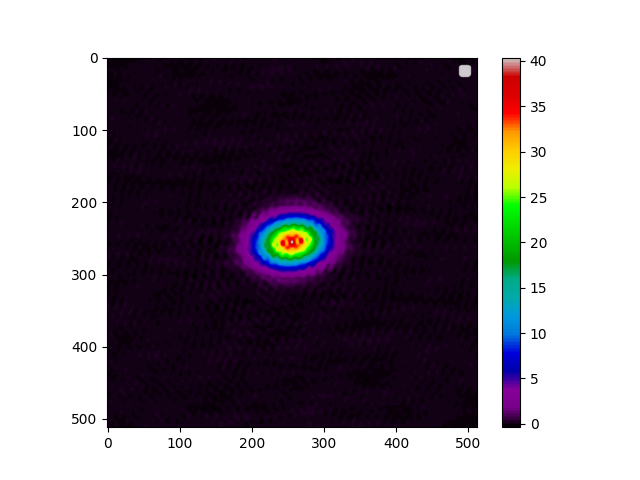
\includegraphics[width=0.5\textwidth]{images/sim_p2_long_color.png}}
    \vspace{0.3cm}
  \subfloat[Residuos Original]{
   \label{fig:clean_residual_clean_3iter}
    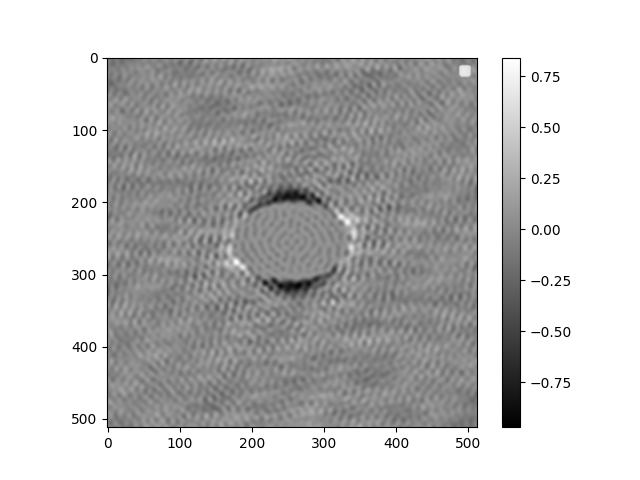
\includegraphics[width=0.5\textwidth]{images/sim_p2_long_residual.png}}
  \subfloat[Residuos Color]{
   \label{fig:clean_residual_color_3iter}
    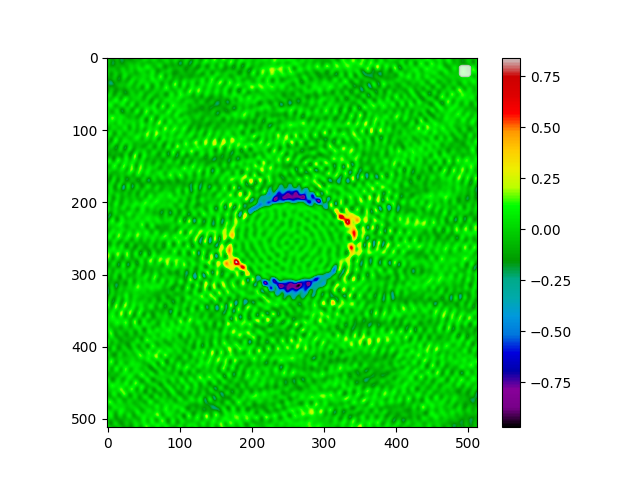
\includegraphics[width=0.5\textwidth]{images/sim_p2_long_color_residual.png}}
 \caption[Tercera iteración para conjunto de datos simulado CLEAN (\textit{long-baseline})]{Tercera iteración para conjunto de datos simulado CLEAN (\textit{long-baseline}). Fuente: Elaboración propia.}
 \label{fig:phasecal_3iter}
\end{figure}

\begin{figure}[!ht]
 \centering
  \subfloat[Original]{
   \label{fig:gpuvmem_original_3iter}
    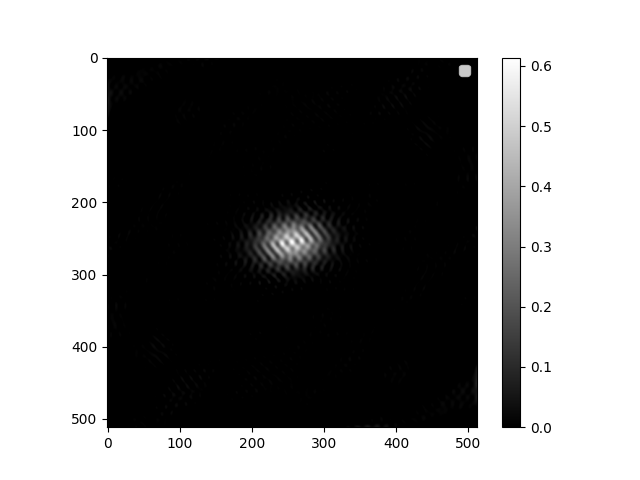
\includegraphics[width=0.5\textwidth]{images/sim_p2_long_gpuvmem.png}}
  \subfloat[Color]{
   \label{fig:gpuvmem_color_3iter}
    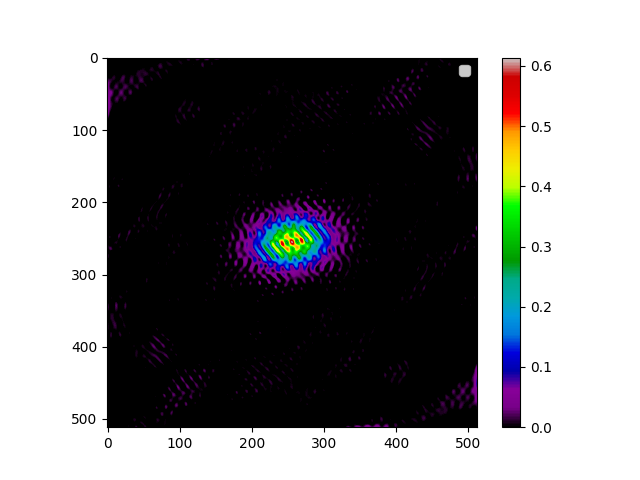
\includegraphics[width=0.5\textwidth]{images/sim_p2_long_gpuvmem_color.png}}
    \vspace{0.3cm}
  \subfloat[Residuos Original]{
   \label{fig:gpuvmem_original_3iter_residual}
    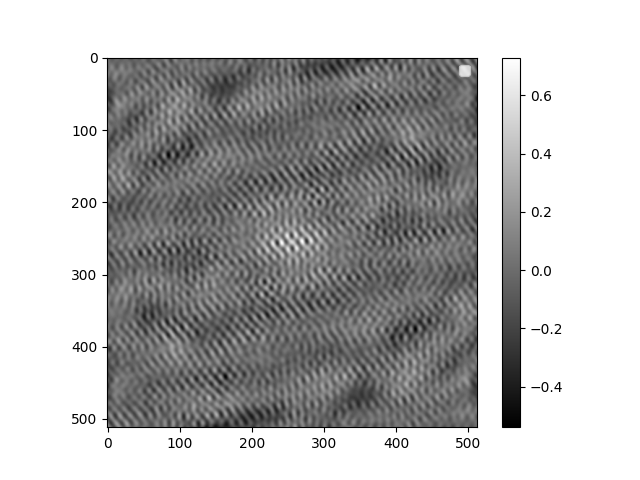
\includegraphics[width=0.5\textwidth]{images/sim_p2_long_gpuvmem_residual.png}}
  \subfloat[Residuos Color]{
   \label{fig:gpuvmem_color_3iter_residual}
    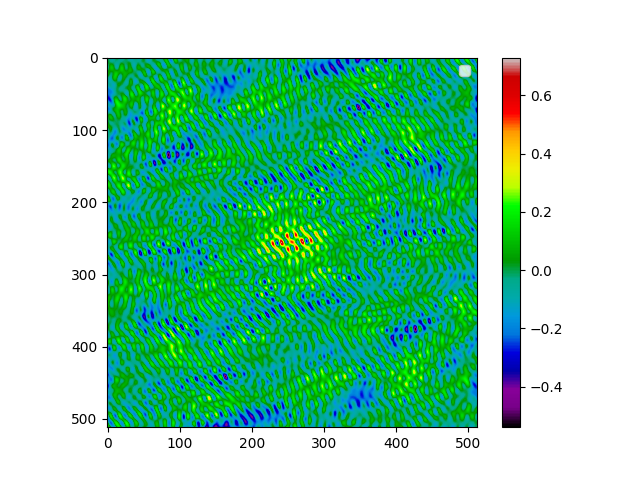
\includegraphics[width=0.5\textwidth]{images/sim_p2_long_gpuvmem_color_residual.png}}
 \caption[Tercera iteración para conjunto de datos simulado GPUVMEM (\textit{long-baseline})]{Tercera iteración para conjunto de datos simulado GPUVMEM (\textit{long-baseline}). Fuente: Elaboración propia.}
 \label{fig:phasecal_3iter_gpuvmem}
\end{figure}

Una cuarta iteración de calibración de fase se realiza considerando un rango de tiempo de 30 segundos, manteniendo la antena de referencia. La Figura \ref{fig:phasecal_4iter} muestra las imágenes reconstruidas y sus residuos mediante el método CLEAN, por otro lado en la Figura \ref{fig:phasecal_4iter_gpuvmem} se ve las imágenes reconstruidas y su residuo. Los valores PSNR para la primera imagen es de 222.6623 y su NRMSE es 0.986208, mientras que para la segunda su PSNR es 220.1864 y su NRMSE 0.763954. 


\begin{figure}[!ht]
 \centering
  \subfloat[Original]{
   \label{fig:clean_original_clean_4iter}
    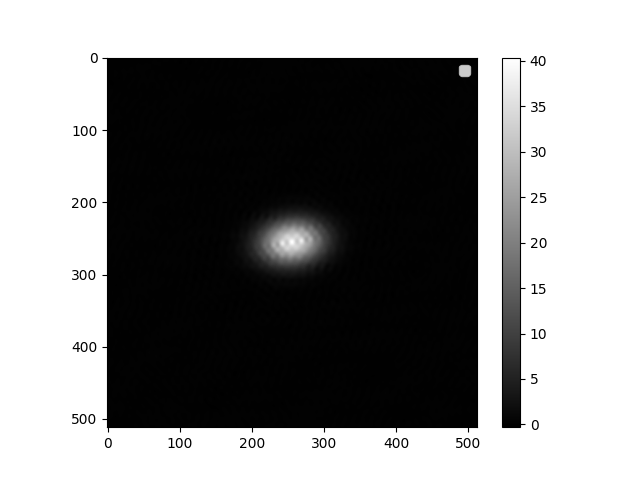
\includegraphics[width=0.5\textwidth]{images/sim_p3_long.png}}
  \subfloat[Color]{
   \label{fig:clean_original_color_4iter}
    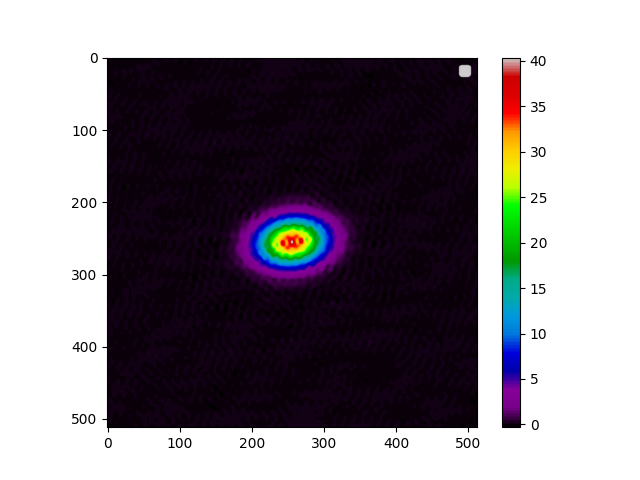
\includegraphics[width=0.5\textwidth]{images/sim_p3_long_color.png}}
    \vspace{0.3cm}
  \subfloat[Residuos Original]{
   \label{fig:clean_residual_clean_4iter}
    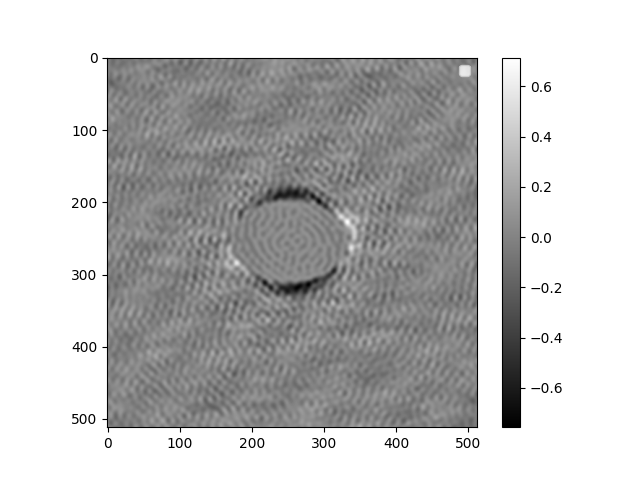
\includegraphics[width=0.5\textwidth]{images/sim_p3_long_residual.png}}
  \subfloat[Residuos Color]{
   \label{fig:clean_residual_color_4iter}
    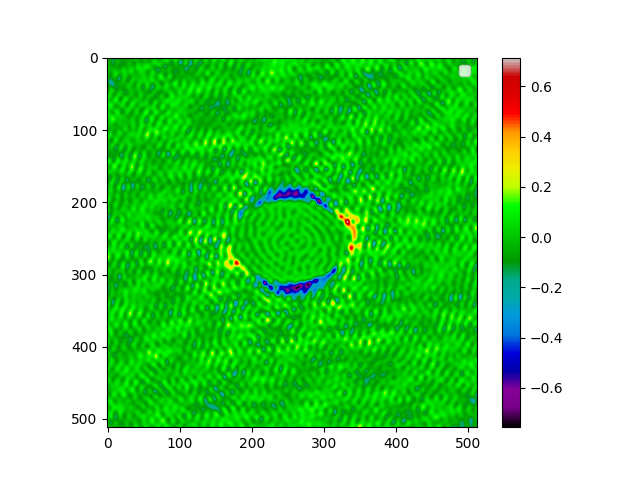
\includegraphics[width=0.5\textwidth]{images/sim_p3_long_color_residual.png}}
 \caption[Cuarta iteración para conjunto de datos simulado CLEAN (\textit{long-baseline})]{Cuarta iteración para conjunto de datos simulado CLEAN (\textit{long-baseline}). Fuente: Elaboración propia.}
 \label{fig:phasecal_4iter}
\end{figure}

\begin{figure}[!ht]
 \centering
  \subfloat[Original]{
   \label{fig:gpuvmem_original_4iter}
    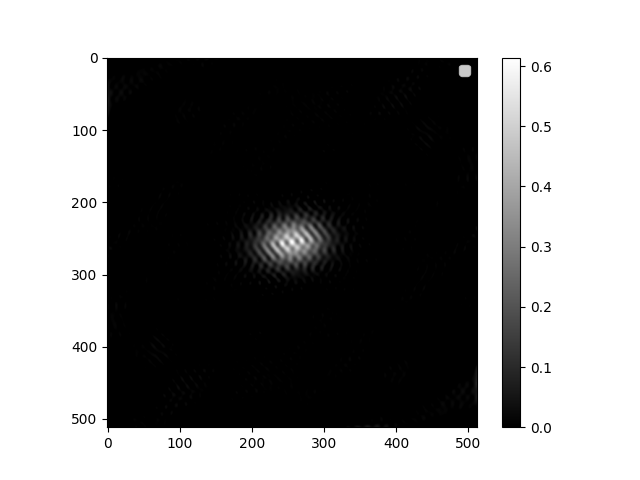
\includegraphics[width=0.5\textwidth]{images/sim_p3_long_gpuvmem.png}}
  \subfloat[Color]{
   \label{fig:gpuvmem_color_4iter}
    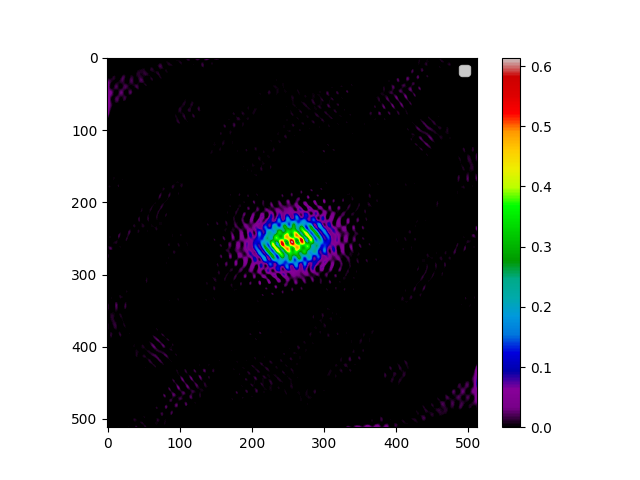
\includegraphics[width=0.5\textwidth]{images/sim_p3_long_gpuvmem_color.png}}
    \vspace{0.3cm}
  \subfloat[Residuos Original]{
   \label{fig:gpuvmem_original_4iter_residual}
    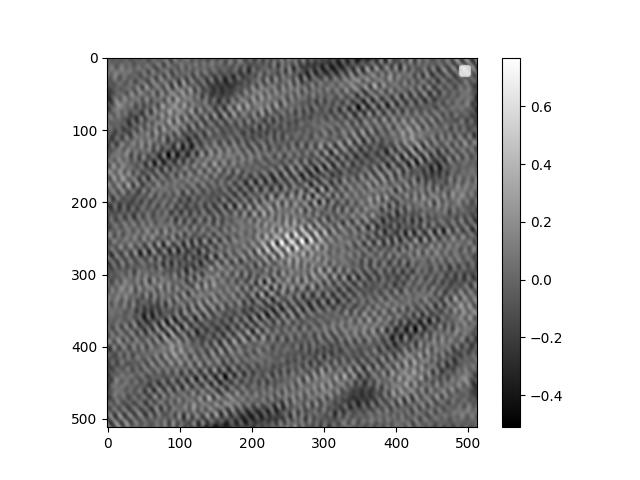
\includegraphics[width=0.5\textwidth]{images/sim_p3_long_gpuvmem_residual.png}}
  \subfloat[Residuos Color]{
   \label{fig:gpuvmem_color_4iter_residual}
    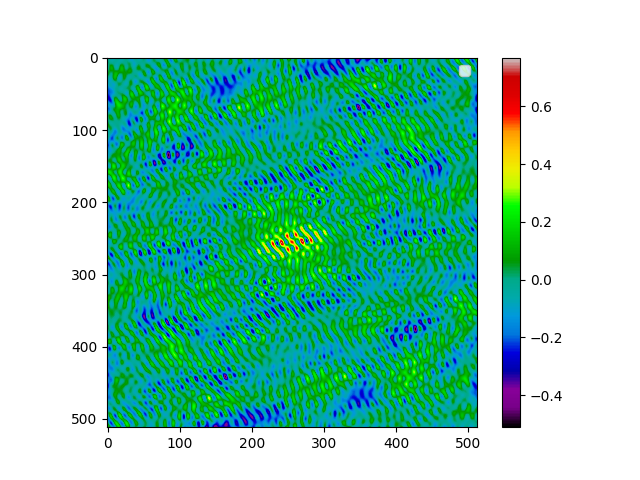
\includegraphics[width=0.5\textwidth]{images/sim_p3_long_gpuvmem_color_residual.png}}
 \caption[Cuarta iteración para conjunto de datos simulado GPUVMEM (\textit{long-baseline})]{Cuarta iteración para conjunto de datos simulado GPUVMEM (\textit{long-baseline}). Fuente: Elaboración propia.}
 \label{fig:phasecal_4iter_gpuvmem}
\end{figure}

La quinta iteración también considera una calibración de fase pero con un rango de tiempo de 18 segundos, donde se sigue manteniendo la antena de referencia. En la Figura \ref{fig:phasecal_5iter} se observa los resultados obtenidos con el método CLEAN donde su PSNR tiene un valor de 219.3188 y su NRMSE de 0.986208. Por otro lado la Figura \ref{fig:phasecal_5iter_gpuvmem} se observa el resultado obtenido con MEM, donde su PSNR tiene un valor de 225.1549  y su NRMSE es de 0.706844.

\begin{figure}[!ht]
 \centering
  \subfloat[Original]{
   \label{fig:clean_original_clean_5iter}
    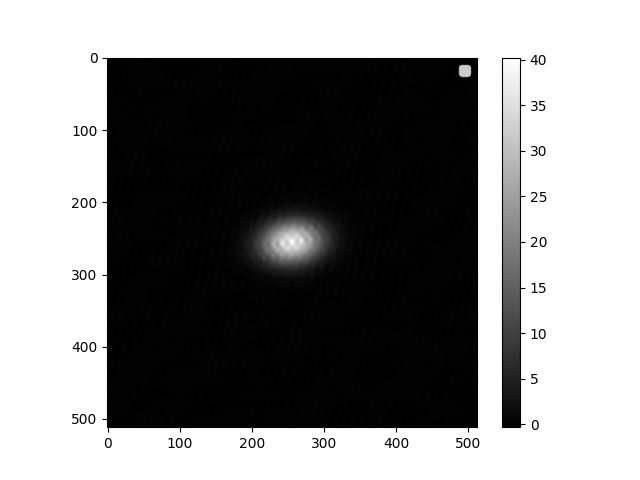
\includegraphics[width=0.5\textwidth]{images/sim_p4_long.png}}
  \subfloat[Color]{
   \label{fig:clean_original_color_5iter}
    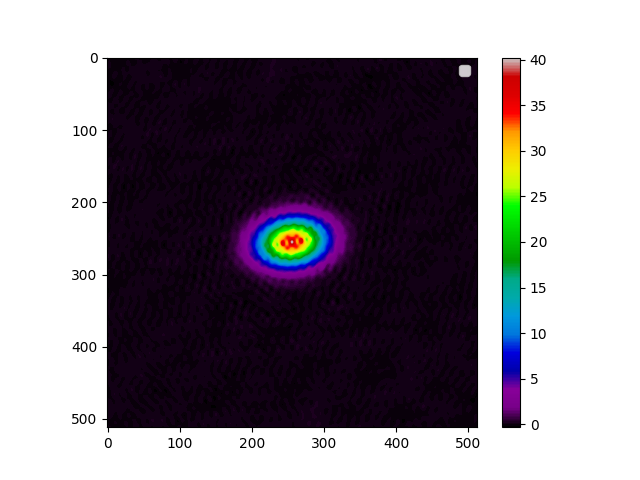
\includegraphics[width=0.5\textwidth]{images/sim_p4_long_color.png}}
    \vspace{0.3cm}
  \subfloat[Residuos Original]{
   \label{fig:clean_residual_clean_5iter}
    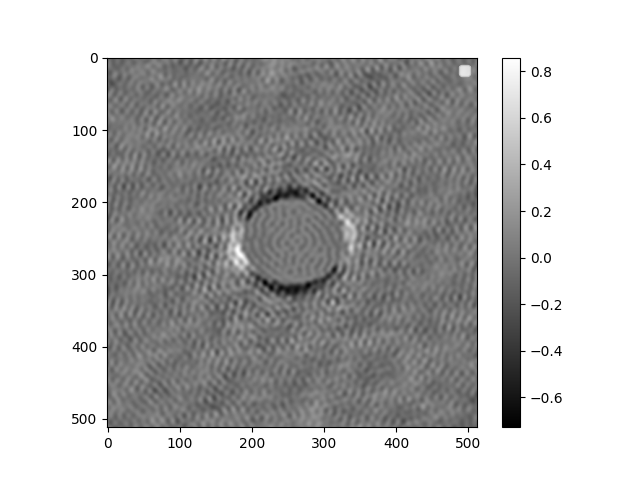
\includegraphics[width=0.5\textwidth]{images/sim_p4_long_residual.png}}
  \subfloat[Residuos Color]{
   \label{fig:clean_residual_color_5iter}
    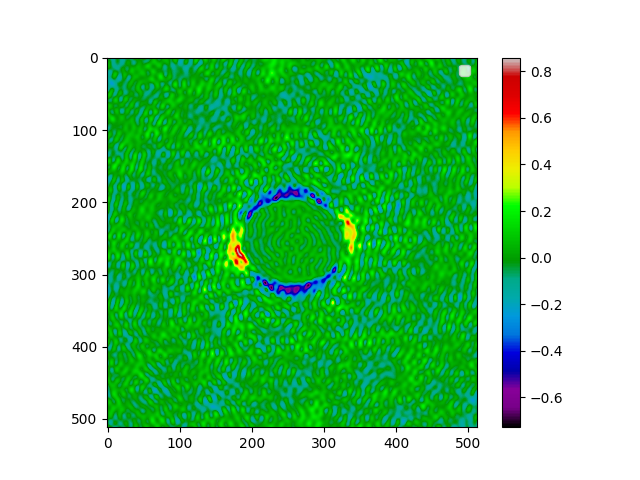
\includegraphics[width=0.5\textwidth]{images/sim_p4_long_color_residual.png}}
 \caption[Quinta iteración para conjunto de datos simulado CLEAN (\textit{long-baseline})]{Quinta iteración para conjunto de datos simulado CLEAN (\textit{long-baseline}). Fuente: Elaboración propia.}
 \label{fig:phasecal_5iter}
\end{figure}

\begin{figure}[!ht]
 \centering
  \subfloat[Original]{
   \label{fig:gpuvmem_original_5iter}
    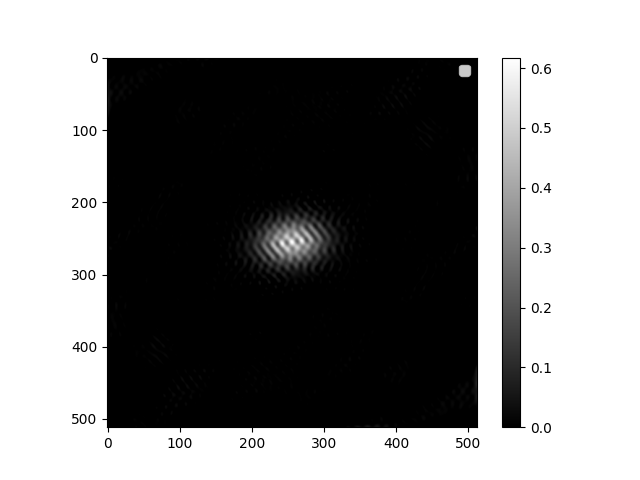
\includegraphics[width=0.5\textwidth]{images/sim_p4_long_gpuvmem.png}}
  \subfloat[Color]{
   \label{fig:gpuvmem_color_5iter}
    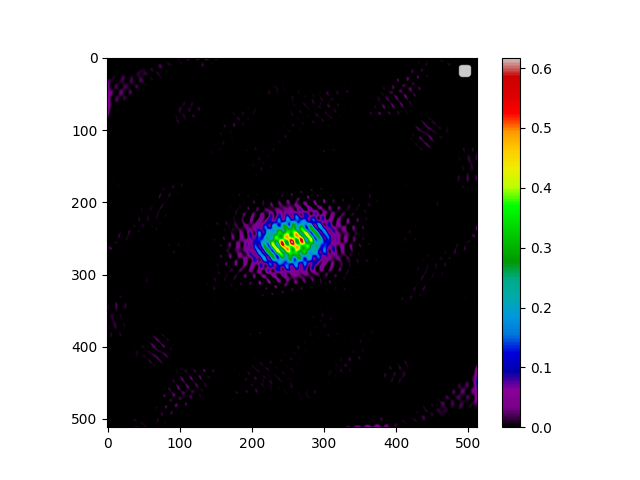
\includegraphics[width=0.5\textwidth]{images/sim_p4_long_gpuvmem_color.png}}
    \vspace{0.3cm}
  \subfloat[Residuos Original]{
   \label{fig:gpuvmem_original_5iter_residual}
    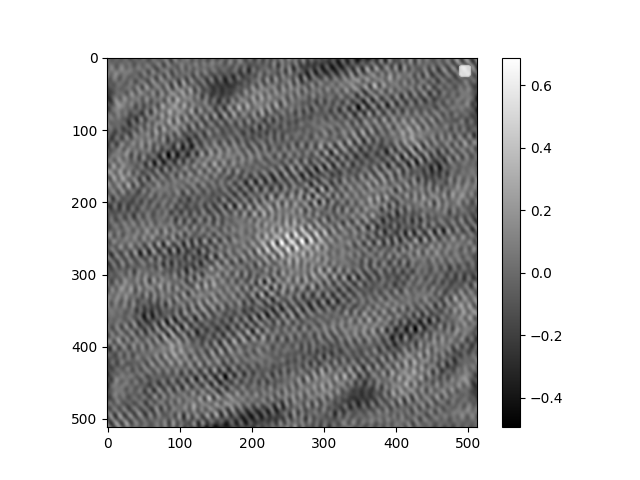
\includegraphics[width=0.5\textwidth]{images/sim_p4_long_gpuvmem_residual.png}}
  \subfloat[Residuos Color]{
   \label{fig:gpuvmem_color_5iter_residual}
    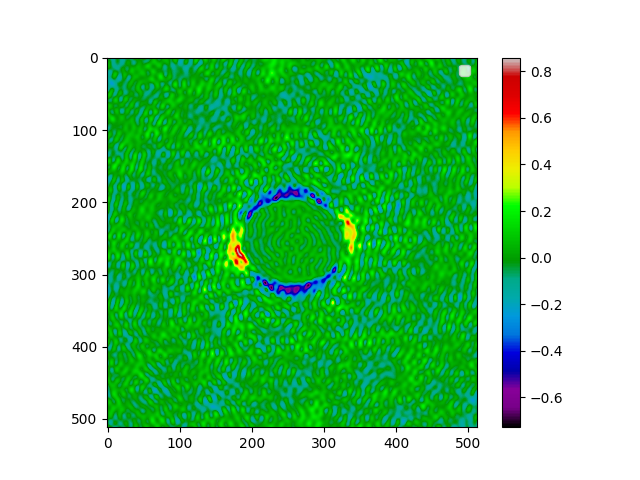
\includegraphics[width=0.5\textwidth]{images/sim_p4_long_color_residual.png}}
 \caption[Quinta iteración para conjunto de datos simulado GPUVMEM (\textit{long-baseline})]{Quinta iteración para conjunto de datos simulado GPUVMEM (\textit{long-baseline}). Fuente: Elaboración propia.}
 \label{fig:phasecal_5iter_gpuvmem}
\end{figure}

Una sexta y última iteración se realiza pero esta vez tanto en amplitud y fase, considerando un tiempo designado como \texttt{inf}, que quiere decir que se realiza por \textit{scan\_number}. La imagen reconstruida con CLEAN se puede ver en la Figura \ref{fig:phasecal_6ter} que tiene un PSNR de 217.0193 y un NRMSE de 0.986210, por otro lado la imagen reconstruida con MEM se puede observar en la Figura \ref{fig:phasecal_6iter_gpuvmem} done esta tiene un PSNR de 219.5513 y un NRMSE de 0.705273. 

\begin{figure}[!ht]
 \centering
  \subfloat[Original]{
   \label{fig:clean_original_clean_6iter}
    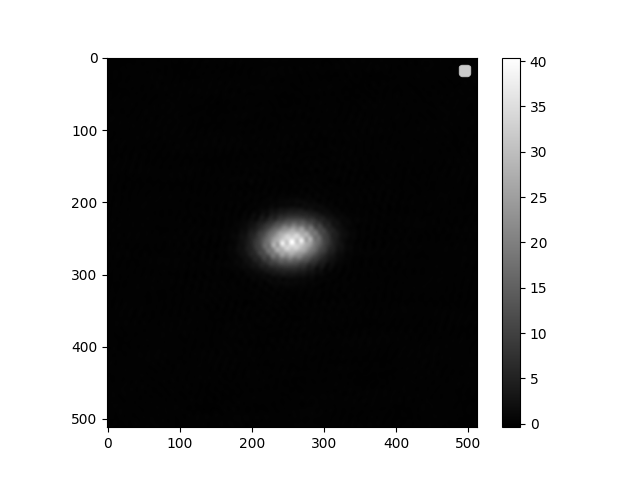
\includegraphics[width=0.5\textwidth]{images/sim_p5_long.png}}
  \subfloat[Color]{
   \label{fig:clean_original_color_6iter}
    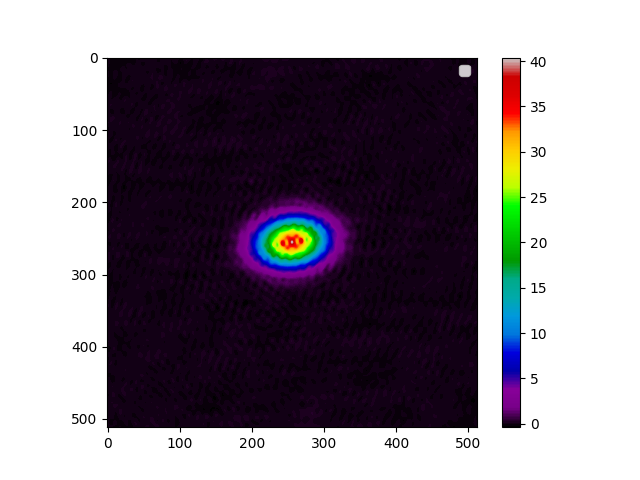
\includegraphics[width=0.5\textwidth]{images/sim_p5_long_color.png}}
    \vspace{0.3cm}
  \subfloat[Residuos Original]{
   \label{fig:clean_residual_clean_6iter}
    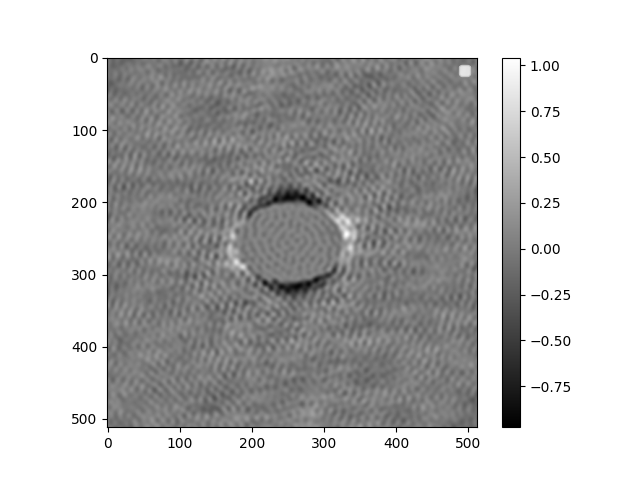
\includegraphics[width=0.5\textwidth]{images/sim_p5_long_residual.png}}
  \subfloat[Residuos Color]{
   \label{fig:clean_residual_color_6iter}
    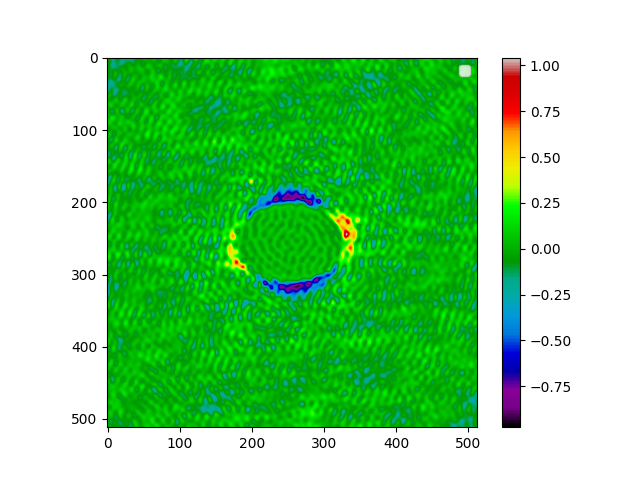
\includegraphics[width=0.5\textwidth]{images/sim_p5_long_color_residual.png}}
 \caption[Sexta iteración para conjunto de datos simulado CLEAN (\textit{long-baseline})]{Sexta iteración para conjunto de datos simulado CLEAN (\textit{long-baseline}). Fuente: Elaboración propia.}
 \label{fig:phasecal_6ter}
\end{figure}

\begin{figure}[!ht]
 \centering
  \subfloat[Original]{
   \label{fig:gpuvmem_original_6iter}
    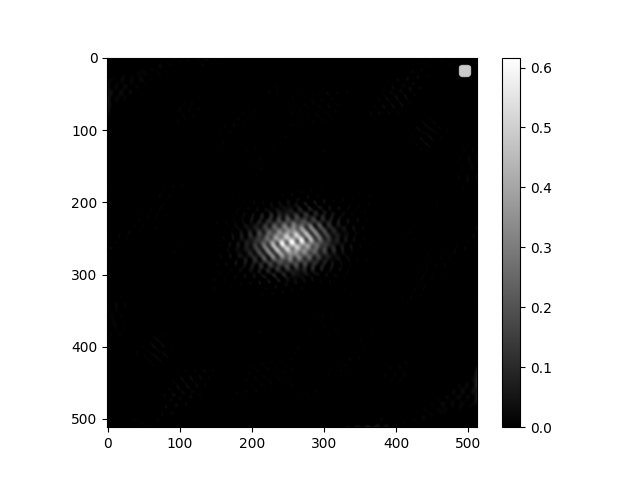
\includegraphics[width=0.5\textwidth]{images/sim_p5_long_gpuvmem.png}}
  \subfloat[Color]{ 
   \label{fig:gpuvmem_color_6iter}
    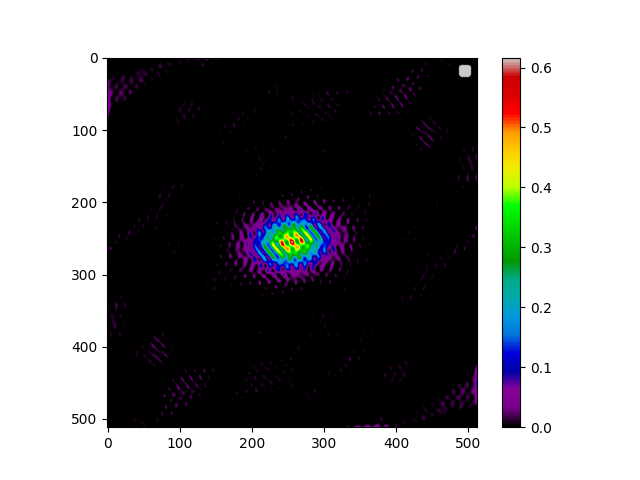
\includegraphics[width=0.5\textwidth]{images/sim_p5_long_gpuvmem_color.png}}
    \vspace{0.3cm}
  \subfloat[Residuos Original]{
   \label{fig:gpuvmem_original_6iter_residual}
    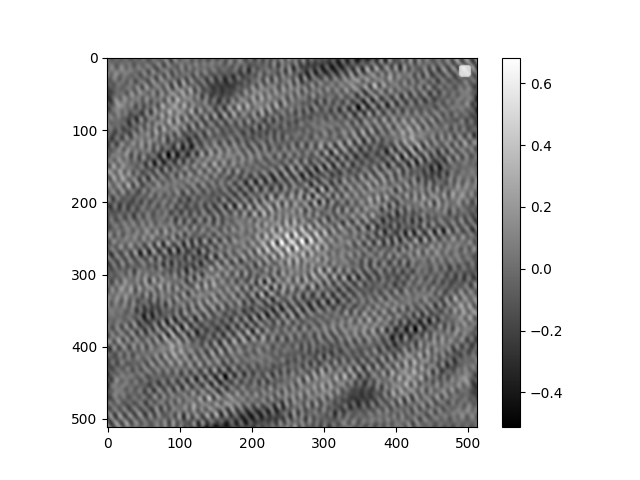
\includegraphics[width=0.5\textwidth]{images/sim_p5_long_gpuvmem_residual.png}}
  \subfloat[Residuos Color]{
   \label{fig:gpuvmem_color_6iter_residual}
    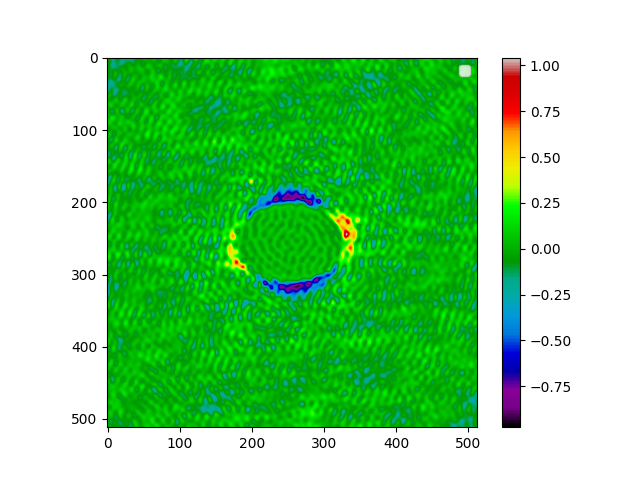
\includegraphics[width=0.5\textwidth]{images/sim_p5_long_color_residual.png}}
 \caption[Sexta iteración para conjunto de datos simulado GPUVMEM (\textit{long-baseline})]{Sexta iteración para conjunto de datos simulado GPUVMEM (\textit{long-baseline}). Fuente: Elaboración propia.}
 \label{fig:phasecal_6iter_gpuvmem}
\end{figure}


En la tabla \ref{tab:sim_long_selfcal_psnr} se puede observar un resumen de los valores para el PSNR de las iteraciones mostradas anteriormente, mientras que en la tabla \ref{tab:sim_long_selfcal_nrmse} se puede observar una tabla resumen con los valores de NRMSE obtenidos para las distintas iteraciones. 

\begin{table}[!ht]
	\begin{center}
		\caption{Tabla con PSNR para \textit{self-calibration} de datos simulados \textit{long-baseline}.}
		\begin{tabular}{| c | c | c |}
			\hline
			Iteración & CLEAN & MEM\\ \hline
			Primera & 218.1818 & 219.3238\\ \hline
            Segunda & 224.1047 & 218.4566\\ \hline
            Tercera & 217.3753 & 218.0049\\ \hline
            Cuarta & 222.6623 & 220.1864\\ \hline
            Quinta & 219.3188 & 225.1549\\ \hline
            Sexta & 217.0193 & 219.5513\\ \hline
		\end{tabular}
		\label{tab:sim_long_selfcal_psnr}
	\end{center}
	\begin{center}
		Fuente: Elaboración propia.
	\end{center}
\end{table}

\begin{table}[!ht]
	\begin{center}
		\caption{Tabla con NRMSE para \textit{self-calibration} de datos simulados \textit{long-baseline}.}
		\begin{tabular}{| c | c | c |}
			\hline
			Iteración & CLEAN & MEM\\ \hline
			Primera & 0.986209 & 0.705504\\ \hline
            Segunda & 0.986204 & 0.706291\\ \hline
            Tercera & 0.986206 & 0.706730\\ \hline
            Cuarta & 0.986203 & 0.763954\\ \hline
            Quinta & 0.986208 & 0.706844\\ \hline
            Sexta & 0.986210 & 0.705273\\ \hline
		\end{tabular}
		\label{tab:sim_long_selfcal_nrmse}
	\end{center}
	\begin{center}
		Fuente: Elaboración propia.
	\end{center}
\end{table}

\subsubsection{\textit{Short-baseline}}

Al igual que en el caso anterior las visibilidades asociado al conjunto de datos vienen perturbadas por una ganancia aleatoria, donde existe una ganancia para cada antena. De esta manera también se escoge una antena de referencia para perturbar solamente las visibilidades asociadas a está antena, para el cual en este caso la antena seleccionada es la DA63. La imagen de este conjunto de datos perturbado puede ser vista en la Figura \ref{fig:dirty_short_baseline}. 

\begin{figure}[!ht]
 \centering
  \subfloat[Original]{
   \label{fig:dirty_original_short}
    \includegraphics[width=0.5\textwidth]{images/noisy_14ant.png}}
  \subfloat[Color]{
   \label{fig:color_original_short}
    \includegraphics[width=0.5\textwidth]{images/noisy_14ant_color.png}}
 \caption[Imagen simulada afectada por una fase (\textit{short-baseline})]{Imagen simulada afectada por una fase (\textit{short-baseline}) Fuente: Elaboración propia.}
 \label{fig:dirty_short_baseline}
\end{figure}

La primera iteración se realiza el método de \textit{self-calibration} en la fase, en la cual se considera una duración de 0 segundos para el rango de tiempo. La Figura \ref{fig:short_sim_p0} muestra la imagen resultante del método CLEAN y la Figura \ref{fig:short_sim_p0_gpuvmem} muestra el resultado mediante el método de MEM, con sus residuos respectivos. Para la imagen con CLEAN se obtuvo un PSNR de 28.7411 y un NRMSE de 0.988454, en cambio para la obtenida con MEM se obtuvo un PSNR de 53.9672 y un NRMSE de 1.012773. 

\begin{figure}[!ht]
 \centering
  \subfloat[Original]{
   \label{fig:short_p0_original}
    \includegraphics[width=0.5\textwidth]{images/short_p0_original.png}}
  \subfloat[Color]{
   \label{fig:short_p0_color}
    \includegraphics[width=0.5\textwidth]{images/short_p0_color.png}}
\vspace{0.3cm}
    \subfloat[Residuos Original]{
   \label{fig:short_p0_original_residual}
    \includegraphics[width=0.5\textwidth]{images/short_p0_original_residual.png}}
  \subfloat[Residuos Color]{
   \label{fig:short_p0_color_residual}
    \includegraphics[width=0.5\textwidth]{images/short_p0_color_residual.png}}
 \caption[Primera iteración para conjunto de datos simulado CLEAN (\textit{short-baseline})]{Primera iteración para conjunto de datos simulado CLEAN (\textit{short-baseline}) Fuente: Elaboración propia.}
 \label{fig:short_sim_p0}
\end{figure}

\begin{figure}[!ht]
 \centering
  \subfloat[Original]{
   \label{fig:short_p0_original_gpuvmem}
    \includegraphics[width=0.5\textwidth]{images/sim_p0_long_gpuvmem.png}}
  \subfloat[Color]{
   \label{fig:short_p0_color_gpuvmem}
    \includegraphics[width=0.5\textwidth]{images/sim_p0_short_gpuvmem_color.png}}
\vspace{0.3cm}
    \subfloat[Residuos Original]{
   \label{fig:short_p0_original_residual_gpuvmem}
    \includegraphics[width=0.5\textwidth]{images/sim_p0_short_gpuvmem_residual.png}}
  \subfloat[Residuos Color]{
   \label{fig:short_p0_color_residual_gpuvmem}
    \includegraphics[width=0.5\textwidth]{images/sim_p0_short_gpuvmem_residual_color.png}}
 \caption[Primera iteración para conjunto de datos simulado MEM (\textit{short-baseline})]{Primera iteración para conjunto de datos simulado MEM (\textit{short-baseline}) Fuente: Elaboración propia.}
 \label{fig:short_sim_p0_gpuvmem}
\end{figure}

Una segunda iteración es realizada pero esta vez mediante el método de \textit{self-calibration} en la amplitud, considerando una duración de 60 segundos para el rango de tiempo. La imagen resultante mediante el método CLEAN para esta segunda iteración puede ser vista en la Figura \ref{fig:short_sim_p1} donde se obtuvo un PSNR de 28.7418 además de un NRMSE de 0.988429 y mediante el método de MEM puede ser vista en la Figura \ref{fig:short_sim_p1_gpuvmem} donde se obtuvo un PSNRE de 51.1989 y un NRMSE de 1.002735. 

\begin{figure}[!ht]
 \centering
  \subfloat[Original]{
   \label{fig:short_p1_original}
    \includegraphics[width=0.5\textwidth]{images/short_p1_original.png}}
  \subfloat[Color]{
   \label{fig:short_p1_color}
    \includegraphics[width=0.5\textwidth]{images/short_p1_color.png}}
\vspace{0.3cm}
    \subfloat[Residuos Original]{
   \label{fig:short_p1_original_residual}
    \includegraphics[width=0.5\textwidth]{images/short_p1_original_residual.png}}
  \subfloat[Residuos Color]{
   \label{fig:short_p1_color_residual}
    \includegraphics[width=0.5\textwidth]{images/short_p1_color_residual.png}}
 \caption[Segunda iteración para conjunto de datos simulado CLEAN (\textit{short-baseline})]{Segunda iteración para conjunto de datos simulado CLEAN (\textit{short-baseline}) Fuente: Elaboración propia.}
 \label{fig:short_sim_p1}
\end{figure}

\begin{figure}[!ht]
 \centering
  \subfloat[Original]{
   \label{fig:short_p1_original_gpuvmem}
    \includegraphics[width=0.5\textwidth]{images/sim_p1_short_gpuvmem.png}}
  \subfloat[Color]{
   \label{fig:short_p1_color_gpuvmem}
    \includegraphics[width=0.5\textwidth]{images/sim_p1_short_gpuvmem_color.png}}
\vspace{0.3cm}
    \subfloat[Residuos Original]{
   \label{fig:short_p1_original_residual_gpuvmem}
    \includegraphics[width=0.5\textwidth]{images/sim_p1_long_gpuvmem_residual.png}}
  \subfloat[Residuos Color]{
   \label{fig:short_p1_color_residual_gpuvmem}
    \includegraphics[width=0.5\textwidth]{images/sim_p1_short_gpuvmem_residual_color.png}}
 \caption[Segunda iteración para conjunto de datos simulado MEM (\textit{short-baseline})]{Segunda iteración para conjunto de datos simulado MEM (\textit{short-baseline}) Fuente: Elaboración propia.}
 \label{fig:short_sim_p1_gpuvmem}
\end{figure}


\begin{table}[!ht]
	\begin{center}
		\caption{Tabla con PSNR para \textit{self-calibration} de datos simulados \textit{short-baseline}.}
		\begin{tabular}{| c | c | c |}
			\hline
			Iteración & CLEAN & MEM\\ \hline
			Primera & 28.7411 & 53.9672\\ \hline
            Segunda & 28.7418 & 51.1989\\ \hline
		\end{tabular}
		\label{tab:sim_short_selfcal_psnr}
	\end{center}
	\begin{center}
		Fuente: Elaboración propia.
	\end{center}
\end{table}


\begin{table}[!ht]
	\begin{center}
		\caption{Tabla con NRMSE para \textit{self-calibration} de datos simulados \textit{short-baseline}.}
		\begin{tabular}{| c | c | c |}
			\hline
			Iteración & CLEAN & MEM\\ \hline
			Primera & 0.988454 & 1.012773\\ \hline
            Segunda & 0.988429 & 1.002735\\ \hline
		\end{tabular}
		\label{tab:sim_short_selfcal_nrmse}
	\end{center}
	\begin{center}
		Fuente: Elaboración propia.
	\end{center}
\end{table}

\subsection{Bispectrum}

Como se menciona en el capitulo \ref{cap:marco}, el método de \textit{Bispectrum} no se ve afectado por la fase, por lo que una prueba a realizar para verificar que la implementación da un buen resultado es comparar resultados entre un conjunto de datos afectado por una fase aleatoria y otro que no. Si la implementación es correcta, el resultado de \textit{Bispectrum} para ambas daría el mismo resultado.

Es así que la prueba a realizar es ejecutar el código con un conjunto de datos afectados por una fase aleatoria y luego ejecutar con un conjunto de datos que no fue afectado por una fase. Para aplicar esta fase se toma en consideración que aquellas visibilidades con misma antena deben ser afectadas por la misma fase, por lo que se generan visibilidades por antena y no por visibilidad. La ecuación utilizada para aplicar la fase es la siguiente, donde los $\theta_{i}$ y $\theta_{j}$ son ángulos aleatorios asociados a una antena $i$ y $j$ respectivamente. 

\begin{equation}
    V_{ij}' = V_{ij}*e^{2i\pi(\theta_{j} - \theta_{i})}
\end{equation}

Para realizar una prueba sencilla se escogerá una fuente puntual para realizar la prueba, es decir que todas las visibilidades del conjunto de datos asociado será uno. De esta manera, según las pruebas ejecutadas, el resultado del conjunto \textit{Bispectrum} sigue siendo uno, tanto para las visibilidades afectadas como las que no, por lo que se cumple la condición principal del método \textit{Bispectrum}.

\subsection{Chi cuadrado bispectrum}

La función de $\chi^{2}$ se puede verificar que se esté comportando de manera correcta al momento de ver los resultados que se obtienen de la ecuación $\chi^{2}(I - \alpha \nabla I)$, de está manera se va cambiando los parámetros de $\chi^{2}$  al realizar una variación en el valor de $\alpha$. De esto se espera que los valores resultantes vayan disminuyendo hasta un cierto punto, indicando así que la función si está minimizando hasta un valor. 

Para la prueba se construyo un conjunto de datos simulado donde la imagen de este objeto puede ser vista en el Figura FIGURA. Por otro lado, se tomo un total de 150 valores distinto de $\alpha$ lo cuales tienen una distancia determinada entre cada valor, por lo que en la Figura \ref{fig:chi2_comp} se puede ver unos gráficos representando el valor de $\alpha$ versus el valor resultante de $\chi^{2}$. Cabe destacar que se realizaron las pruebas con distintos valores para la distancia entre los valores de $\alpha$.

\begin{figure}
 \centering
  \subfloat[Distancia entre $\alpha$ de 1e-8]{
   \label{fig:1e8}
    \includegraphics[width=0.32\textwidth]{images/chi2_result_8.jpg}}
  \subfloat[Distancia entre $\alpha$ de 1e-9]{
   \label{fig:1e9}
    \includegraphics[width=0.32\textwidth]{images/chi2_result_9.jpg}}
  \subfloat[Distancia entre $\alpha$ de 1e-10]{
   \label{fig:1e10}
    \includegraphics[width=0.32\textwidth]{images/chi2_result_10.jpg}}
 \caption[Comportamiento de $\chi^{2}$.]{Comportamiento de $\chi^{2}$. Fuente: Elaboración propia.}
 \label{fig:chi2_comp}
\end{figure}

El gradiente presentado en el capitulo \ref{sec:bispectrum} (ecuación \ref{eq:derivadaBis}) se puede probar comparando el resultado de esta con la imagen sucia del conjunto de datos y si esta está correcta estas dos imágenes serán similares. Para esto se utiliza igualmente el conjunto de datos simulado presentado en la figura \ref{fig:simulated_image} dando como resultado lo que se muestra en la figura \ref{fig:grad_sim}. Si bien hay diferencias, estos tienen similitudes lo que da a entender que el gradiente del \textit{bispectrum} ofrece una buena aproximación. 

\begin{figure}[!ht]
	\centering
	\captionsetup{justification=centering}
	\includegraphics[scale=0.45]{images/grad_sim.png}
	\caption[Gradiente de conjunto de datos simulado]{Gradiente de conjunto de datos simulado. Fuente: Elaboración propia}
	\label{fig:grad_sim}
\end{figure}

\section{Datos reales}


\subsection{Self-calibration}

Los siguientes experimentos fueron realizados utilizando los conjuntos de datos HD163296 reducidos que fueron creados en la sección \ref{sec:datos_reducidos} por la misma razón explicada en esa sección. Al igual que los datos simulados, los parámetros escogidos para calibrar y el método de CLEAN son sacados del script proporcionado por DSHARP. Al contrario que en el caso anterior, en esta no se realiza una perturbación del conjunto de datos. La imágenes sucias de los conjuntos de datos puede ser vista en la Figura \ref{fig:hd163296_obs3} para \textit{short-baseline} y  Figura \ref{fig:hd163296_obs8} para \textit{long-baseline}.

\subsubsection{\textit{Long-baseline}}

Para una primera iteración se considera una calibración de fase la cual tiene un tiempo de rango de 360 segundos. En la Figura \ref{fig:real_clean_p0} se observa la imagen reconstruida con CLEAN que tiene un PSNR de 67.4770 y un 0.118788. La figura \ref{fig:real_p0_gpuvmem} muestra el resultado obtenido con MEM donde este tiene un PSNR de 19.2603 y un NRMSE de 73.14086.

\begin{figure}[!ht]
 \centering
  \subfloat[Original]{
   \label{fig:real_clean_p0}
    \includegraphics[width=0.45\textwidth]{images/HD163296_p0_long.png}}
  \subfloat[Color]{
   \label{fig:real_clean_p0_color}
    \includegraphics[width=0.45\textwidth]{images/HD163296_p0_long_color.png}}
    \vspace{0.3cm}
  \subfloat[Residuos Original]{
   \label{fig:real_clean_p0_residual}
    \includegraphics[width=0.45\textwidth]{images/HD163296_p0_long_residual.png}}
  \subfloat[Residuos Color]{
   \label{fig:reak_clean_p0_residual_color}
    \includegraphics[width=0.45\textwidth]{images/HD163296_p0_long_color_residual.png}}
 \caption[Primera iteración para conjunto de datos HD163296 CLEAN (\textit{long-baseline})]{Primera iteración para conjunto de datos HD163296 CLEAN (\textit{long-baseline}). Fuente: Elaboración propia.}
 \label{fig:real_p0_clean}
\end{figure}

\begin{figure}[!ht]
 \centering
  \subfloat[Original]{
   \label{fig:real_gpuvmem_p0}
    \includegraphics[width=0.45\textwidth]{images/HD163296_p0_long_gpuvmem.png}}
  \subfloat[Color]{
   \label{fig:real_gpuvmem_p0_color}
    \includegraphics[width=0.45\textwidth]{images/HD163296_p0_long_gpuvmem_color.png}}
    \vspace{0.3cm}
  \subfloat[Original]{
   \label{fig:real_gpuvmem_p0_residual}
    \includegraphics[width=0.45\textwidth]{images/HD163296_p0_long_gpuvmem_residual.png}}
  \subfloat[Color]{
   \label{fig:real_gpuvmem_p0_residual_color}
    \includegraphics[width=0.45\textwidth]{images/HD163296_p0_long_gpuvmem_color_residual.png}}
 \caption[Primera iteración para conjunto de datos simulado GPUVMEM (\textit{long-baseline})]{Primera iteración para conjunto de datos simulado GPUVMEM (\textit{long-baseline}). Fuente: Elaboración propia.}
 \label{fig:real_p0_gpuvmem}
\end{figure}

Una segunda iteración se realiza para calibrar en la fase nuevamente donde se utiliza un tiempo de 120 segundos. La Figura \ref{fig:real_p1_clean} es el resultado obtenido con CLEAN que tiene un PSNR de 67.4688 y un NRMSE de 0.119099, donde por otro lado se tiene la Figura \ref{fig:real_p1_gpuvmem} muestra el resultado con MEM que tiene un PSNR de 19.2607 y un NRMSE de 73.141163.

\begin{figure}[!ht]
 \centering
  \subfloat[Original]{
   \label{fig:real_clean_p1}
    \includegraphics[width=0.45\textwidth]{images/HD163296_p1_long.png}}
  \subfloat[Color]{
   \label{fig:real_clean_p1_color}
    \includegraphics[width=0.45\textwidth]{images/HD163296_p1_long_color.png}}
    \vspace{0.3cm}
  \subfloat[Residuos Original]{
   \label{fig:real_clean_p1_residual}
    \includegraphics[width=0.45\textwidth]{images/HD163296_p1_long_residual.png}}
  \subfloat[Residuos Color]{
   \label{fig:reak_clean_p1_residual_color}
    \includegraphics[width=0.45\textwidth]{images/HD163296_p1_long_color_residual.png}}
 \caption[Segunda iteración para conjunto de datos HD163296 CLEAN (\textit{long-baseline})]{Segunda iteración para conjunto de datos HD163296 CLEAN (\textit{long-baseline}). Fuente: Elaboración propia.}
 \label{fig:real_p1_clean}
\end{figure}

\begin{figure}[!ht]
 \centering
  \subfloat[Original]{
   \label{fig:real_gpuvmem_p1}
    \includegraphics[width=0.45\textwidth]{images/HD163296_p1_long_gpuvmem.png}}
  \subfloat[Color]{
   \label{fig:real_gpuvmem_p1_color}
    \includegraphics[width=0.45\textwidth]{images/HD163296_p1_long_gpuvmem_color.png}}
    \vspace{0.3cm}
  \subfloat[Original]{
   \label{fig:real_gpuvmem_p1_residual}
    \includegraphics[width=0.45\textwidth]{images/HD163296_p1_long_gpuvmem_residual.png}}
  \subfloat[Color]{
   \label{fig:real_gpuvmem_p1_residual_color}
    \includegraphics[width=0.45\textwidth]{images/HD163296_p1_long_gpuvmem_color_residual.png}}
 \caption[Segunda iteración para conjunto de datos simulado GPUVMEM (\textit{long-baseline})]{Segunda iteración para conjunto de datos simulado GPUVMEM (\textit{long-baseline}). Fuente: Elaboración propia.}
 \label{fig:real_p1_gpuvmem}
\end{figure}

La tercera iteración en fase realizada se considera un tiempo de 60 segundos. En la Figura \ref{fig:real_p2_clean} se observa el resultado con CLEAN que obtiene un PSNR de 68.8393 y un NRMSE 0.117767, por otro lado en la Figura \ref{fig:real_p2_gpuvmem} se muestra el resultado obtenido con MEM donde se obtiene un PSNR de 19.2318 y un NRMSE de 73.142270.

\begin{figure}[!ht]
 \centering
  \subfloat[Original]{
   \label{fig:real_clean_p2}
    \includegraphics[width=0.45\textwidth]{images/HD163296_p2_long.png}}
  \subfloat[Color]{
   \label{fig:real_clean_p2_color}
    \includegraphics[width=0.45\textwidth]{images/HD163296_p2_long_color.png}}
    \vspace{0.3cm}
  \subfloat[Residuos Original]{
   \label{fig:real_clean_p2_residual}
    \includegraphics[width=0.45\textwidth]{images/HD163296_p2_long_residual.png}}
  \subfloat[Residuos Color]{
   \label{fig:reak_clean_p2_residual_color}
    \includegraphics[width=0.45\textwidth]{images/HD163296_p2_long_color_residual.png}}
 \caption[Tercera iteración para conjunto de datos HD163296 CLEAN (\textit{long-baseline})]{Tercera iteración para conjunto de datos HD163296 CLEAN (\textit{long-baseline}). Fuente: Elaboración propia.}
 \label{fig:real_p2_clean}
\end{figure}

\begin{figure}[!ht]
 \centering
  \subfloat[Original]{
   \label{fig:real_gpuvmem_p2}
    \includegraphics[width=0.45\textwidth]{images/HD163296_p2_long_gpuvmem.png}}
  \subfloat[Color]{
   \label{fig:real_gpuvmem_p2_color}
    \includegraphics[width=0.45\textwidth]{images/HD163296_p2_long_gpuvmem_color.png}}
    \vspace{0.3cm}
  \subfloat[Original]{
   \label{fig:real_gpuvmem_p2_residual}
    \includegraphics[width=0.45\textwidth]{images/HD163296_p2_long_gpuvmem_residual.png}}
  \subfloat[Color]{
   \label{fig:real_gpuvmem_p2_residual_color}
    \includegraphics[width=0.45\textwidth]{images/HD163296_p2_long_gpuvmem_color_residual.png}}
 \caption[Tercera iteración para conjunto de datos simulado GPUVMEM (\textit{long-baseline})]{Tercera iteración para conjunto de datos simulado GPUVMEM (\textit{long-baseline}). Fuente: Elaboración propia.}
 \label{fig:real_p2_gpuvmem}
\end{figure}

Una cuarta iteración se realiza en la fase con un rango de tiempo de 30 segundos. En la Figura \ref{fig:real_p3_clean} se ve el resultado obtenido con CLEAN con un PSNR de 67.5953 y un NRMSE 0.1186669, en cambio en la Figura \ref{fig:real_p3_gpuvmem} es el resultado obtenido con MEM, donde este tiene un PSNR de 19.2318 y un NRMSE de 73.169250.

\begin{figure}[!ht]
 \centering
  \subfloat[Original]{
   \label{fig:real_clean_p3}
    \includegraphics[width=0.45\textwidth]{images/HD163296_p3_long.png}}
  \subfloat[Color]{
   \label{fig:real_clean_p3_color}
    \includegraphics[width=0.45\textwidth]{images/HD163296_p3_long_color.png}}
    \vspace{0.3cm}
  \subfloat[Residuos Original]{
   \label{fig:real_clean_p3_residual}
    \includegraphics[width=0.45\textwidth]{images/HD163296_p3_long_residual.png}}
  \subfloat[Residuos Color]{
   \label{fig:reak_clean_p3_residual_color}
    \includegraphics[width=0.45\textwidth]{images/HD163296_p3_long_color_residual.png}}
 \caption[Cuarta iteración para conjunto de datos HD163296 CLEAN (\textit{long-baseline})]{Segunda iteración para conjunto de datos HD163296 CLEAN (\textit{long-baseline}). Fuente: Elaboración propia.}
 \label{fig:real_p3_clean}
\end{figure}

\begin{figure}[!ht]
 \centering
  \subfloat[Original]{
   \label{fig:real_gpuvmem_p3}
    \includegraphics[width=0.45\textwidth]{images/HD163296_p3_long_gpuvmem.png}}
  \subfloat[Color]{
   \label{fig:real_gpuvmem_p3_color}
    \includegraphics[width=0.45\textwidth]{images/HD163296_p3_long_gpuvmem_color.png}}
    \vspace{0.3cm}
  \subfloat[Original]{
   \label{fig:real_gpuvmem_p3_residual}
    \includegraphics[width=0.45\textwidth]{images/HD163296_p3_long_gpuvmem_residual.png}}
  \subfloat[Color]{
   \label{fig:real_gpuvmem_p3_residual_color}
    \includegraphics[width=0.45\textwidth]{images/HD163296_p3_long_gpuvmem_color_residual.png}}
 \caption[Cuarta iteración para conjunto de datos simulado GPUVMEM (\textit{long-baseline})]{Cuarta iteración para conjunto de datos simulado GPUVMEM (\textit{long-baseline}). Fuente: Elaboración propia.}
 \label{fig:real_p3_gpuvmem}
\end{figure}

La quinta iteración en fase se realiza considerando un tiempo de 18 segundos. En la Figura \ref{fig:real_p4_clean} se observa el resultado con CLEAN que obtiene un PSNR de 68.4272 y un NRMSE de 0.118262, en cambio el resultado obtenido con MEM se puede observar en la Figura \ref{fig:real_p4_gpuvmem} que tiene un PSNR de 19.2637 y un NRMSE de 73.148380.

\begin{figure}[!ht]
 \centering
  \subfloat[Original]{
   \label{fig:real_clean_p4}
    \includegraphics[width=0.45\textwidth]{images/HD163296_p4_long.png}}
  \subfloat[Color]{
   \label{fig:real_clean_p4_color}
    \includegraphics[width=0.45\textwidth]{images/HD163296_p4_long_color.png}}
    \vspace{0.3cm}
  \subfloat[Residuos Original]{
   \label{fig:real_clean_p4_residual}
    \includegraphics[width=0.45\textwidth]{images/HD163296_p4_long_residual.png}}
  \subfloat[Residuos Color]{
   \label{fig:reak_clean_p4_residual_color}
    \includegraphics[width=0.45\textwidth]{images/HD163296_p4_long_color_residual.png}}
 \caption[Quinta iteración para conjunto de datos HD163296 CLEAN (\textit{long-baseline})]{Quinta iteración para conjunto de datos HD163296 CLEAN (\textit{long-baseline}). Fuente: Elaboración propia.}
 \label{fig:real_p4_clean}
\end{figure}

\begin{figure}[!ht]
 \centering
  \subfloat[Original]{
   \label{fig:real_gpuvmem_p4}
    \includegraphics[width=0.45\textwidth]{images/HD163296_p4_long_gpuvmem.png}}
  \subfloat[Color]{
   \label{fig:real_gpuvmem_p4_color}
    \includegraphics[width=0.45\textwidth]{images/HD163296_p4_long_gpuvmem_color.png}}
    \vspace{0.3cm}
  \subfloat[Original]{
   \label{fig:real_gpuvmem_p4_residual}
    \includegraphics[width=0.45\textwidth]{images/HD163296_p4_long_gpuvmem_residual.png}}
  \subfloat[Color]{
   \label{fig:real_gpuvmem_p4_residual_color}
    \includegraphics[width=0.45\textwidth]{images/HD163296_p4_long_gpuvmem_color_residual.png}}
 \caption[Quinta iteración para conjunto de datos simulado GPUVMEM (\textit{long-baseline})]{Quinta iteración para conjunto de datos simulado GPUVMEM (\textit{long-baseline}). Fuente: Elaboración propia.}
 \label{fig:real_p4_gpuvmem}
\end{figure}

Finalmente una sexta iteración es realizada en fase y amplitud considerando un tiempo \texttt{inf}, es decir la calibración se realiza por \texttt{scan\_number}. El resultado obtenido con CLEAN se puede observar en la Figura \ref{fig:real_p5_clean} donde se obtiene un PSNR de 68.8455 y un NRMSE de 0.120623, por otro lado el resultado obtenido con MEM se muestra en la Figura \ref{fig:real_p5_gpuvmem} que tiene un PSNR de 68.8455 y un NRMS de 19.2886.

\begin{figure}[!ht]
 \centering
  \subfloat[Original]{
   \label{fig:real_clean_p5}
    \includegraphics[width=0.45\textwidth]{images/HD163296_p5_long.png}}
  \subfloat[Color]{
   \label{fig:real_clean_p5_color}
    \includegraphics[width=0.45\textwidth]{images/HD163296_p5_long_color.png}}
    \vspace{0.3cm}
  \subfloat[Residuos Original]{
   \label{fig:real_clean_p5_residual}
    \includegraphics[width=0.45\textwidth]{images/HD163296_p5_long_residual.png}}
  \subfloat[Residuos Color]{
   \label{fig:reak_clean_p5_residual_color}
    \includegraphics[width=0.45\textwidth]{images/HD163296_p5_long_color_residual.png}}
 \caption[Sexta iteración para conjunto de datos HD163296 CLEAN (\textit{long-baseline})]{Sexta iteración para conjunto de datos HD163296 CLEAN (\textit{long-baseline}). Fuente: Elaboración propia.}
 \label{fig:real_p5_clean}
\end{figure}


\begin{figure}[!ht]
 \centering
  \subfloat[Original]{
   \label{fig:real_gpuvmem_p5}
    \includegraphics[width=0.45\textwidth]{images/HD163296_p5_long_gpuvmem.png}}
  \subfloat[Color]{
   \label{fig:real_gpuvmem_p5_color}
    \includegraphics[width=0.45\textwidth]{images/HD163296_p5_long_gpuvmem_color.png}}
    \vspace{0.3cm}
  \subfloat[Original]{
   \label{fig:real_gpuvmem_p5_residual}
    \includegraphics[width=0.45\textwidth]{images/HD163296_p5_long_gpuvmem_residual.png}}
  \subfloat[Color]{
   \label{fig:real_gpuvmem_p5_residual_color}
    \includegraphics[width=0.45\textwidth]{images/HD163296_p5_long_gpuvmem_color_residual.png}}
 \caption[Sexta iteración para conjunto de datos simulado GPUVMEM (\textit{long-baseline})]{Sexta iteración para conjunto de datos simulado GPUVMEM (\textit{long-baseline}). Fuente: Elaboración propia.}
 \label{fig:real_p5_gpuvmem}
\end{figure}

En la Tabla \ref{tab:real_long_selfcal_psnr} y en la Tabla \ref{tab:real_long_selfcal_nrmse} se ve un resumen de los resultados obtenidos de las métricas PSNR y NRMSE correspondientemente.

\begin{table}[!ht]
	\begin{center}
		\caption{Tabla con PSNR para \textit{self-calibration} de datos HD163296 \textit{long-baseline}.}
		\begin{tabular}{| c | c | c |}
			\hline
			Iteración & CLEAN & MEM\\ \hline
			Primera & 67.4770 & 19.2603\\ \hline
            Segunda & 67.4688 & 19.2607\\ \hline
            Tercera & 68.8393 & 19.2596\\ \hline
            Cuarta & 67.5953 & 19.2318\\ \hline
            Quinta & 68.4272 & 19.2637\\ \hline
            Sexta & 68.8455 & 19.2886\\ \hline
		\end{tabular}
		\label{tab:real_long_selfcal_psnr}
	\end{center}
	\begin{center}
		Fuente: Elaboración propia.
	\end{center}
\end{table}

\begin{table}[!ht]
	\begin{center}
		\caption{Tabla con NRMSE para \textit{self-calibration} de datos HD163296 \textit{long-baseline}.}
		\begin{tabular}{| c | c | c |}
			\hline
			Iteración & CLEAN & MEM\\ \hline
			Primera & 0.118788 & 73.140686\\ \hline
            Segunda & 0.119099 & 73.141163\\ \hline
            Tercera & 0.117767 & 73.152270\\ \hline
            Cuarta & 0.118669 & 73.169250\\ \hline
            Quinta & 0.118262 & 73.148380\\ \hline
            Sexta & 0.120623 & 73.138954\\ \hline
		\end{tabular}
		\label{tab:real_long_selfcal_nrmse}
	\end{center}
	\begin{center}
		Fuente: Elaboración propia.
	\end{center}
\end{table}


\subsubsection{\textit{Short-baseline}}

 Una primera iteración en la fase es considerada con un rango de tiempo de 0 segundos. En la Figura \ref{fig:real_short_p0_clean} se puede ver la imagen reconstruida con CLEAN y sus residuos, donde para esta se obtuvo un PSNR de 158.9637 y un NRMSE de 0.0097. La Figura \ref{fig:real_short_p0_mem} muestra la imagen reconstruida con MEM junto a sus residuos, donde se obtuvo un PSNR de 599.8952 y un NRMSE de 84.7032. 

\begin{figure}[!ht]
 \centering
  \subfloat[Original]{
   \label{fig:real_short_clean_p0}
    \includegraphics[width=0.45\textwidth]{images/real_p0_short.png}}
  \subfloat[Color]{
   \label{fig:real_short_clean_p0_color}
    \includegraphics[width=0.45\textwidth]{images/real_p0_short_color.png}}
    \vspace{0.3cm}
  \subfloat[Residuos Original]{
   \label{fig:real_short_clean_p0_residual}
    \includegraphics[width=0.45\textwidth]{images/real_p0_short_residual.png}}
  \subfloat[Residuos Color]{
   \label{fig:real_short_clean_p0_residual_color}
    \includegraphics[width=0.45\textwidth]{images/real_p0_short_color_residual.png}}
 \caption[Primera iteración para conjunto de datos HD163296 CLEAN (\textit{short-baseline})]{Primera iteración para conjunto de datos HD163296 CLEAN (\textit{short-baseline}). Fuente: Elaboración propia.}
 \label{fig:real_short_p0_clean}
\end{figure}

\begin{figure}[!ht]
 \centering
  \subfloat[Original]{
   \label{fig:real_short_mem_p0}
    \includegraphics[width=0.45\textwidth]{images/real_p0_short_gpuvmem.png}}
  \subfloat[Color]{
   \label{fig:real_short_mem_p0_color}
    \includegraphics[width=0.45\textwidth]{images/real_p0_short_gpuvmem_color.png}}
    \vspace{0.3cm}
  \subfloat[Residuos Original]{
   \label{fig:real_short_mem_p0_residual}
    \includegraphics[width=0.45\textwidth]{images/real_p0_short_gpuvmem_residual.png}}
  \subfloat[Residuos Color]{
   \label{fig:real_short_mem_p0_residual_color}
    \includegraphics[width=0.45\textwidth]{images/real_p0_short_gpuvmem_color_residual.png}}
 \caption[Primera iteración para conjunto de datos HD163296 MEM (\textit{short-baseline})]{Primera iteración para conjunto de datos HD163296 MEM (\textit{short-baseline}). Fuente: Elaboración propia.}
 \label{fig:real_short_p0_mem}
\end{figure}

Una segunda iteración se realiza una calibración de fase y amplitud considerando un tiempo de 60 segundos. En la Figura \ref{fig:real_short_p1_clean} se observa el resultado la reconstrucción con el método CLEAN que obtiene un PSNR de 152.5449 y un NRMSE de 0.0026, en cambio, en la Figura \ref{fig:real_short_p1_mem} se observa reconstruida con el método MEM que tiene un PSNR de 627.0048 y un NRMSE de 84.5635. 

\begin{figure}[!ht]
 \centering
  \subfloat[Original]{
   \label{fig:real_short_clean_p1}
    \includegraphics[width=0.45\textwidth]{images/real_p1_short.png}}
  \subfloat[Color]{
   \label{fig:real_short_clean_p1_color}
    \includegraphics[width=0.45\textwidth]{images/real_p1_short_color.png}}
    \vspace{0.3cm}
  \subfloat[Residuos Original]{
   \label{fig:real_short_clean_p1_residual}
    \includegraphics[width=0.45\textwidth]{images/real_p1_short_residual.png}}
  \subfloat[Residuos Color]{
   \label{fig:real_short_clean_p1_residual_color}
    \includegraphics[width=0.45\textwidth]{images/real_p1_short_color_residual.png}}
 \caption[Segunda iteración para conjunto de datos HD163296 CLEAN (\textit{short-baseline})]{Segunda iteración para conjunto de datos HD163296 CLEAN (\textit{short-baseline}). Fuente: Elaboración propia.}
 \label{fig:real_short_p1_clean}
\end{figure}

\begin{figure}[!ht]
 \centering
  \subfloat[Original]{
   \label{fig:real_short_mem_p1}
    \includegraphics[width=0.45\textwidth]{images/real_p1_short_gpuvmem.png}}
  \subfloat[Color]{
   \label{fig:real_short_mem_p1_color}
    \includegraphics[width=0.45\textwidth]{images/real_p1_short_gpuvmem_color.png}}
    \vspace{0.3cm}
  \subfloat[Residuos Original]{
   \label{fig:real_short_mem_p1_residual}
    \includegraphics[width=0.45\textwidth]{images/real_p1_short_gpuvmem_residual.png}}
  \subfloat[Residuos Color]{
   \label{fig:real_short_mem_p1_residual_color}
    \includegraphics[width=0.45\textwidth]{images/real_p1_short_gpuvmem_color_residual.png}}
 \caption[Segunda iteración para conjunto de datos HD163296 MEM (\textit{short-baseline})]{Segunda iteración para conjunto de datos HD163296 MEM (\textit{short-baseline}). Fuente: Elaboración propia.}
 \label{fig:real_short_p1_mem}
\end{figure}

En la tabla \ref{tab:real_short_selfcal_psnr} se ve un resumen de los resultados obtenidos de la métrica PSNR y en la tabla \ref{tab:real_short_selfcal_nrmse} se observa un resumen de los resultados obtenidos para la métrica NRMSE. 

\begin{table}[!ht]
	\begin{center}
		\caption{Tabla con PSNR para \textit{self-calibration} de HD163296 \textit{short-baseline}.}
		\begin{tabular}{| c | c | c |}
			\hline
			Iteración & CLEAN & MEM\\ \hline
			Primera & 148.9637 & 599.8952\\ \hline
            Segunda & 152.5449 & 627.0048\\ \hline
		\end{tabular}
		\label{tab:real_short_selfcal_psnr}
	\end{center}
	\begin{center}
		Fuente: Elaboración propia.
	\end{center}
\end{table}


\begin{table}[!ht]
	\begin{center}
		\caption{Tabla con NRMSE para \textit{self-calibration} de HD163296 \textit{short-baseline}.}
		\begin{tabular}{| c | c | c |}
			\hline
			Iteración & CLEAN & MEM\\ \hline
			Primera & 0.0097 & 84.7032\\ \hline
            Segunda & 0.0026 & 84.5635\\ \hline
		\end{tabular}
		\label{tab:real_short_selfcal_nrmse}
	\end{center}
	\begin{center}
		Fuente: Elaboración propia.
	\end{center}
\end{table}

\begin{comment}

\section{\textit{Self-calibration}}

Las pruebas realizadas con este métodos se utilizaron algunos de los conjuntos de datos proporcionados por DSharp (CITAR), donde estos fueron calibrados en fase, amplitud y ambas juntas. El proceso para obtener la imágenes se realiza mediante la generación de una imagen modelo mediante GPUVMEM y luego se aplica el método \textit{self-calibration}. 

\subsection{Fase}

El primer set de datos utilizado es el llamado GWLup en su versión continua. Para la primera iteración se considera como antena de referencia DV18 y un rango de tiempo de 30 segundos. Una comparación entre la imagen sin \textit{self-calibration} y aquella obtenida luego de una iteración de \textit{self-calibration} puede ser observada en la Figura \ref{fig:phase1}.


\begin{figure}[!ht]
	\centering
	\captionsetup{justification=centering}
	\includegraphics[scale=0.15]{images/original_1iter_gw.png}
	\caption[Primera iteración de GWLup con \textit{self-calibration} de fase]{Imagen original (izquierda) y resultado primera iteración de \textit{self-calibration} para GWLup (derecha). Fuente: Elaboración propia}
	\label{fig:phase1}
\end{figure}

%Al analizar el resultado de la primera iteración se puede ver que existe una mejora aunque difícil de percibir de manera rápida, sin embargo existen detalles mejor definidos como es el caso de los discos exteriores que se ven mas marcados que en su versión sin calibrar. Aún así, al calcular la métrica de PSNR se puede ver que este aumenta con respecto al original, pasando desde 84.1969 a 90.2997 indicando que el ruido disminuyo en la imagen resultante. 

La siguiente iteración se realizo tomando como entrada el set de datos generado en la iteración anterior, sin embargo, el rango de tiempo utilizado para esta iteración es de 18 segundos y se mantiene la antena de referencia. El resultado de esta iteración se puede ver en la Figura \ref{fig:phase2}.  

\begin{figure}[!ht]
	\centering
	\captionsetup{justification=centering}
	\includegraphics[scale=0.15]{images/1iter_2iter_gw.png}
	\caption[Segunda iteración de GWLup con \textit{self-calibration} de fase]{Primera iteración (izquierda) y resultado segunda iteración de \textit{self-calibration} para GWLup (derecha). Fuente: Elaboración propia}
	\label{fig:phase2}
\end{figure}

Una ultima iteración es hecha con el parámetro de tiempo inf, donde se toma el set de datos producido en la iteración anterior y se sigue manteniendo la misma antena de referencia. De esto se obtiene como resultado lo visto en la Figura \ref{fig:phase3}.

\begin{figure}[!ht]
	\centering
	\captionsetup{justification=centering}
	\includegraphics[scale=0.15]{images/1iter_2iter_gw.png}
	\caption[Tercera iteración de GWLup con \textit{self-calibration} de fase]{Segunda iteración (izquierda) y resultado tercera iteración de \textit{self-calibration} para GWLup (derecha). Fuente: Elaboración propia}
	\label{fig:phase3}
\end{figure}

Para obtener una mejor referencia al momento de comparar y analizar imágenes, se muestra en la siguiente tabla resumen el valor correspondiente para la métrica PSNR en cada una de las iteraciones, donde la iteración 0 corresponde a la imagen original sin \textit{self-calibration}. Así también en la figura \ref{fig:phaseAll} se presenta el resumen de las imagenes resultantes de las iteraciones. 


\begin{table}[!ht]
	\begin{center}
		\caption{Tabla con PSNR para \textit{self-calibration} de fase.}
		\begin{tabular}{| c | c | c | c |}
			\hline
			Iteración & Antena & Tiempo [s] & PSNR\\ \hline
			0 & -- & -- & 235.7107\\ \hline
            1 & DV18 & 30 & 272.4133\\ \hline
            2 & DV18 & 18 & 244.1781\\ \hline
            3 & DV18 & inf & 227.9313\\ \hline
		\end{tabular}
		\label{tab:fase}
	\end{center}
	\begin{center}
		Fuente: Elaboración propia.
	\end{center}
\end{table}

\begin{figure}[!ht]
	\centering
	\captionsetup{justification=centering}
	\includegraphics[scale=0.15]{images/all_gw.png}
	\caption[Proceso de \textit{self-calibraiton} para GWLup con \textit{self-calibration} de fase]{Imagen original (izquierda superior), primera iteración (derecha superior), segunda iteración (izquierda inferior) y tercera iteración (derecha inferior)}
	\label{fig:phaseAll}
\end{figure}


Sin embargo, en el experimento anterior se realizan iteraciones con tiempos pequeños por lo que también se realiza un experimento con rangos de tiempo mas grandes. La primera iteración tiene un rango de tiempo de 900 segundos y como antena de referencia la DV18. El resultado se puede ver en la figura \ref{fig:phase1900}.

\begin{figure}[!ht]
	\centering
	\captionsetup{justification=centering}
	\includegraphics[scale=0.15]{images/origina_1iter900.png}
	\caption[Primera iteración de GWLup con 900 segundos]{Imagen original (izquierda) y resultado primera iteración de \textit{self-calibration} para GWLup (derecha) con 900 segundos. Fuente: Elaboración propia}
	\label{fig:phase1900}
\end{figure}

Una segunda iteración es realizada utilizando un rango de tiempo de 360 segundos 

\begin{table}[!ht]
	\begin{center}
		\caption{Tabla con PSNR para \textit{self-calibration} de fase con mayor rango de tiempo.}
		\begin{tabular}{| c | c | c | c |}
			\hline
			Iteración & Antena & Tiempo [s] & PSNR\\ \hline
			0 & -- & -- & 235.7107\\ \hline
            1 & DV18 & 900 & 265.3531\\ \hline
            2 & DV18 & 360 & 239.0052\\ \hline
            3 & DV18 & 180 & 249.8769\\ \hline
		\end{tabular}
		\label{tab:faseLarge}
	\end{center}
	\begin{center}
		Fuente: Elaboración propia.
	\end{center}
\end{table}


\subsection{Amplitud}

Para estas pruebas también se considera la utilización del conjunto de datos GWLup. La primera iteración se considera a la antena DV18 como referencia y un rango de tiempo de 30 segundos. Cabe destacar que para este experimento se utilizó el conjunto de datos no calibrado como entrada para la primera iteración para así analizar solamente el comportamiento de \textit{self-calibration} de amplitud. El resultado de esta iteración se ve en la Figura \ref{fig:amp1}.

\begin{figure}[!ht]
	\centering
	\captionsetup{justification=centering}
	\includegraphics[scale=0.15]{images/original_1iteramp.png}
	\caption[Primera iteración de GWLup con \textit{self-calibration} de amplitud]{Imagen original (izquierda) y resultado primera iteración de \textit{self-calibration} para GWLup (derecha) de amplitud. Fuente: Elaboración propia}
	\label{fig:amp1}
\end{figure}

Una segunda iteración es realizada manteniendo la antena de referencia pero con un rango de tiempo de unos 18 segundos. Este resultado se ve en la Figura \ref{fig:amp2}.

\begin{figure}[!ht]
	\centering
	\captionsetup{justification=centering}
	\includegraphics[scale=0.15]{images/1iter_2iter_amp_gw.png}
	\caption[Segunda iteración de GWLup con \textit{self-calibration} de amplitud]{Primera iteración (izquierda) y resultado segunda iteración de \textit{self-calibration} para GWLup (derecha). Fuente: Elaboración propia}
	\label{fig:amp2}
\end{figure}

Finalmente una tercera iteración es realizada, donde se vuelve a mantener la antena de referencia y se utiliza un rango de tiempo con valor inf. Este resultado se puede ver representado en la Figura \ref{fig:amp3}.

\begin{figure}[!ht]
	\centering
	\captionsetup{justification=centering}
	\includegraphics[scale=0.15]{images/2iter_3iter_amp_gw.png}
	\caption[Tercera iteración de GWLup con \textit{self-calibration} de amplitud]{Segunda iteración (izquierda) y resultado tercera iteración de \textit{self-calibration} para GWLup (derecha). Fuente: Elaboración propia}
	\label{fig:amp3}
\end{figure}

Al igual que el caso de la fase en algunas imágenes es difícil encontrar una diferencia pero por lo mismo se toman métricas para poder ver si hay alguna mejora o no. En la tabla \ref{tab:amp} se muestra los valores de PSNR obtenidos en cada iteración junto al rango de tiempo y antena utilizadas. Además en la Figura \ref{fig:allamp} se presenta un resumen de las imágenes obtenidas en las iteraciones. 

\begin{table}[!ht]
	\begin{center}
		\caption{Tabla con PSNR para \textit{self-calibration} de amplitud.}
		\begin{tabular}{| c | c | c | c |}
			\hline
			Iteración & Antena & Tiempo [s] & PSNR\\ \hline
			0 & -- & -- & 235.7107\\ \hline
            1 & DV18 & 30 & 237.88065\\ \hline
            2 & DV18 & 18 & 196.33336 \\ \hline
            3 & DV18 & inf & 250.84782\\ \hline
		\end{tabular}
		\label{tab:amp}
	\end{center}
	\begin{center}
		Fuente: Elaboración propia.
	\end{center}
\end{table}

\begin{figure}[!ht]
	\centering
	\captionsetup{justification=centering}
	\includegraphics[scale=0.15]{images/all_amp_gw.png}
	\caption[Proceso de \textit{self-calibration} de amplitud para GWLup]{Imagen original (izquierda superior), primera iteración (derecha superior), segunda iteración (izquierda inferior) y tercera iteración (derecha inferior)}
	\label{fig:allamp}
\end{figure}

\subsection{Fase y Amplitud}

Una combinación entre fase y amplitud también es probada, para este caso se realiza dos iteraciones de fase y una de amplitud, donde se toma el conjunto de datos resultante de la segunda iteración de fase con rangos de tiempos cortos (Figura \ref{fig:phase2}). En cuanto a la iteración en amplitud, se sigue manteniendo la antena de referencia DV18 y se utiliza un tiempo inf. El resultado se presenta en la Figura \ref{fig:phaseAmpGW}.


\begin{figure}[!ht]
	\centering
	\captionsetup{justification=centering}
	\includegraphics[scale=0.15]{images/ph_amp_gw.png}
	\caption[Proceso de \textit{self-calibraiton} de fase y amplitud para GWLup]{Segunda iteración (izquierda) y resultado segunda tercera de \textit{self-calibration} para GWLup (derecha). Fuente: Elaboración propia}
	\label{fig:phaseAmpGW}
\end{figure}


\begin{table}[!ht]
	\begin{center}
		\caption{Tabla con PSNR para \textit{self-calibration} de fase y amplitud.}
		\begin{tabular}{| c | c | c | c | c |}
			\hline
			Iteración & Antena & Tiempo [s] & PSNR & Método\\ \hline
			0 & -- & -- & 235.7107 & --\\ \hline
            1 & DV18 & 30 & 272.4133 & fase\\ \hline
            2 & DV18 & 18 & 244.1781 & fase\\ \hline
            3 & DV18 & inf & 248.8000 & amplitud\\ \hline
		\end{tabular}
		\label{tab:faseAmp}
	\end{center}
	\begin{center}
		Fuente: Elaboración propia.
	\end{center}
\end{table}

\end{comment}




